\documentclass[11pt,a4paper,oneside]{report}

% ============================================================
% 1. CONFIGURACIÓN GENERAL
% ============================================================

\usepackage[utf8]{inputenc}
\usepackage[T1]{fontenc}
\usepackage[spanish,es-tabla]{babel}

\usepackage[expansion=false]{microtype}

\usepackage[
    top=2.7cm,
    bottom=2.5cm,
    left=3cm,
    right=2.5cm
]{geometry}

% ============================================================
% 2. MATEMÁTICAS, FIGURAS Y TABLAS
% ============================================================

\usepackage{amsmath,amssymb}
\usepackage{graphicx}
\usepackage{float}
\usepackage{caption}
\usepackage{subcaption}
\usepackage{booktabs}
\usepackage{tabularx}
\usepackage{longtable}
\usepackage{array}
\usepackage{multirow}
\usepackage[table]{xcolor}

% ============================================================
% 3. DIAGRAMAS
% ============================================================

\usepackage{tikz}

\usetikzlibrary{
    positioning,
    arrows.meta,
    shapes.geometric,
    shapes.misc,
    fit,
    backgrounds,
    calc
}

% ============================================================
% 4. CÓDIGO FUENTE
% ============================================================

\usepackage{listings}

\definecolor{codebackground}{RGB}{245,247,250}
\definecolor{codekeyword}{RGB}{35,75,135}
\definecolor{codestring}{RGB}{30,125,90}
\definecolor{codecomment}{RGB}{110,120,130}
\definecolor{codeborder}{RGB}{215,220,228}

\lstdefinestyle{codestyle}{
    backgroundcolor=\color{codebackground},
    basicstyle=\ttfamily\footnotesize,
    keywordstyle=\color{codekeyword}\bfseries,
    stringstyle=\color{codestring},
    commentstyle=\color{codecomment}\itshape,
    numbers=left,
    numberstyle=\tiny\color{gray},
    stepnumber=1,
    numbersep=10pt,
    breaklines=true,
    breakatwhitespace=false,
    showstringspaces=false,
    frame=single,
    rulecolor=\color{codeborder},
    tabsize=4,
    captionpos=b,
    keepspaces=true,
    columns=fullflexible,
    literate=
        {á}{{\'a}}1 {é}{{\'e}}1 {í}{{\'i}}1 {ó}{{\'o}}1 {ú}{{\'u}}1
        {Á}{{\'A}}1 {É}{{\'E}}1 {Í}{{\'I}}1 {Ó}{{\'O}}1 {Ú}{{\'U}}1
        {ñ}{{\~n}}1 {Ñ}{{\~N}}1 {ü}{{\"u}}1 {Ü}{{\"U}}1
        {¿}{{?`}}1 {¡}{{!`}}1
}

\lstdefinelanguage{yaml}{
    keywords={true,false,null,yes,no,on,off},
    sensitive=true,
    comment=[l]{\#},
    morestring=[b]',
    morestring=[b]"
}

\lstset{style=codestyle}

% ============================================================
% 5. COLORES DEL DOCUMENTO
% ============================================================

\definecolor{reportblue}{RGB}{25,55,90}
\definecolor{reportdark}{RGB}{35,45,58}
\definecolor{reportgray}{RGB}{105,115,125}
\definecolor{reportlight}{RGB}{240,243,247}
\definecolor{reportcyan}{RGB}{35,150,175}
\definecolor{reportred}{RGB}{180,55,55}
\definecolor{reportorange}{RGB}{210,135,35}
\definecolor{reportgreen}{RGB}{50,130,90}

% Colores utilizados por los diagramas y tablas de la primera parte.
\definecolor{gitfeat}{RGB}{35,130,85}
\definecolor{gitfix}{RGB}{180,55,55}
\definecolor{gitdocs}{RGB}{35,120,175}
\definecolor{gitchore}{RGB}{130,95,35}
\definecolor{gitrefactor}{RGB}{115,75,155}
\definecolor{gitmerge}{RGB}{210,135,35}
\definecolor{reportbg}{RGB}{240,243,247}
\definecolor{dockvolume}{RGB}{35,150,175}
\definecolor{netpublic}{RGB}{35,120,175}
\definecolor{netprivate}{RGB}{180,55,55}

% ============================================================
% 6. FORMATO DE TÍTULOS
% ============================================================

\usepackage{titlesec}

\titleformat{\chapter}[display]
    {\normalfont\bfseries\color{reportblue}}
    {\filleft\Large\thechapter}
    {1ex}
    {\titlerule\vspace{1ex}\LARGE}
    [\vspace{1ex}\titlerule]

\titleformat{\section}
    {\normalfont\large\bfseries\color{reportblue}}
    {\thesection}
    {0.8em}
    {}

\titleformat{\subsection}
    {\normalfont\normalsize\bfseries\color{reportdark}}
    {\thesubsection}
    {0.8em}
    {}

\titleformat{\subsubsection}
    {\normalfont\normalsize\bfseries\color{reportdark}}
    {\thesubsubsection}
    {0.8em}
    {}

\titlespacing*{\chapter}{0pt}{-15pt}{25pt}
\titlespacing*{\section}{0pt}{16pt}{7pt}
\titlespacing*{\subsection}{0pt}{12pt}{5pt}

% ============================================================
% 7. ENCABEZADOS Y PIES DE PÁGINA
% ============================================================

\usepackage{fancyhdr}

\pagestyle{fancy}
\fancyhf{}

\fancyhead[L]{\small\color{reportgray} Informe}
\fancyhead[R]{\small\color{reportgray} DevOps / DevSecOps}

\fancyfoot[L]{\small\color{reportgray} Universidad de Ingeniería y Tecnología}
\fancyfoot[R]{\small\color{reportblue}\thepage}

\renewcommand{\headrulewidth}{0.4pt}
\renewcommand{\footrulewidth}{0.4pt}

\fancypagestyle{plain}{
    \fancyhf{}
    \fancyfoot[L]{\small\color{reportgray} Universidad de Ingeniería y Tecnología}
    \fancyfoot[R]{\small\color{reportblue}\thepage}
    \renewcommand{\headrulewidth}{0pt}
}

% ============================================================
% 8. HIPERVÍNCULOS
% ============================================================

\usepackage{hyperref}

\hypersetup{
    colorlinks=true,
    linkcolor=reportblue,
    citecolor=reportblue,
    urlcolor=reportcyan,
    pdftitle={Informe Final del Proyecto DevOps},
    pdfauthor={Equipo de desarrollo},
    pdfsubject={Implementación de DevOps y DevSecOps},
    pdfkeywords={DevOps, DevSecOps, STRIDE, CI/CD, SAST, DAST}
}

% ============================================================
% 9. LISTAS
% ============================================================

\usepackage{enumitem}

\setlist[itemize]{
    leftmargin=1.5cm,
    itemsep=3pt,
    topsep=5pt
}

\setlist[enumerate]{
    leftmargin=1.5cm,
    itemsep=3pt,
    topsep=5pt
}

\setlength{\parindent}{0pt}
\setlength{\parskip}{5pt}

% ============================================================
% 10. CAJAS
% ============================================================

\usepackage[most]{tcolorbox}

\newtcolorbox{infobox}{
    colback=reportlight,
    colframe=reportblue,
    boxrule=0.5pt,
    arc=2mm,
    left=3mm,
    right=3mm,
    top=2mm,
    bottom=2mm
}

\newtcolorbox{warningbox}{
    colback=orange!5,
    colframe=reportorange,
    boxrule=0.5pt,
    arc=2mm,
    left=3mm,
    right=3mm,
    top=2mm,
    bottom=2mm
}

\newtcolorbox{notebox}{
    colback=reportlight,
    colframe=reportcyan,
    boxrule=0.5pt,
    arc=2mm,
    left=3mm,
    right=3mm,
    top=2mm,
    bottom=2mm
}

% ============================================================
% 11. COMANDOS PERSONALIZADOS
% ============================================================

\newcommand{\pendiente}[1]{
    \textcolor{reportred}{\textbf{[PENDIENTE: #1]}}
}

\newcommand{\campo}[1]{
    \textcolor{reportgray}{\textit{#1}}
}

\newcommand{\evidencefigure}[3]{
    \begin{figure}[H]
        \centering

        \IfFileExists{#1}{
            \includegraphics[
                width=0.95\linewidth,
                height=0.55\textheight,
                keepaspectratio
            ]{#1}
        }{
            \fbox{
                \parbox[c][5cm][c]{0.85\linewidth}{
                    \centering
                    \textbf{Evidencia pendiente}\\[3mm]
                    \campo{#1}\\[2mm]
                    \small Insertar figura o captura correspondiente.
                }
            }
        }

        \caption{#2}
        \label{#3}
    \end{figure}
}

\newcommand{\externallink}[2]{
    \href{#1}{\textcolor{reportcyan}{#2}}
}

\setcounter{tocdepth}{0}
% ============================================================
% 12. INICIO DEL DOCUMENTO
% ============================================================

\begin{document}

% ------------------------------------------------------------
% PORTADA
% ------------------------------------------------------------


\begin{titlepage}

% ====================================================
% FONDO AZUL NOCTURNO CON LUNA DIFUSA Y ESTRELLAS
% ====================================================

\begin{tikzpicture}[remember picture, overlay]

    % Fondo azul oscuro con gradiente
    \fill[
        top color=blue!25!black,
        bottom color=blue!8!black
    ]
    (current page.south west)
    rectangle
    (current page.north east);

    % Luna difusa en la esquina superior derecha
    \begin{scope}[
        shift={([xshift=-4.5cm,yshift=-4.5cm]
        current page.north east)}
    ]

        \fill[white, opacity=0.03] (0,0) circle (3.5cm);
        \fill[white, opacity=0.06] (0,0) circle (2.5cm);
        \fill[white, opacity=0.10] (0,0) circle (1.6cm);
        \fill[white, opacity=0.18] (0,0) circle (1.0cm);

        \fill[yellow!15!white, opacity=0.85]
        (0,0) circle (0.65cm);

        \fill[white, opacity=0.95]
        (-0.05,0.05) circle (0.60cm);

    \end{scope}

    % Campo de estrellas
    \foreach \x/\y/\s/\o in {
        0.08/0.92/0.8/0.9,
        0.15/0.85/0.5/0.7,
        0.22/0.95/0.7/0.8,
        0.28/0.78/0.4/0.6,
        0.05/0.65/0.6/0.7,
        0.12/0.48/0.5/0.6,
        0.18/0.32/0.7/0.8,
        0.09/0.15/0.4/0.5,
        0.35/0.88/0.6/0.8,
        0.42/0.96/0.8/0.9,
        0.48/0.82/0.5/0.6,
        0.38/0.60/0.6/0.7,
        0.30/0.42/0.4/0.5,
        0.45/0.25/0.7/0.8,
        0.33/0.12/0.5/0.6,
        0.55/0.90/0.7/0.8,
        0.62/0.82/0.5/0.6,
        0.58/0.68/0.6/0.7,
        0.52/0.45/0.4/0.5,
        0.65/0.30/0.8/0.9,
        0.58/0.15/0.5/0.6,
        0.72/0.94/0.6/0.7,
        0.78/0.80/0.8/0.9,
        0.85/0.88/0.5/0.6,
        0.70/0.65/0.7/0.8,
        0.82/0.52/0.4/0.5,
        0.75/0.35/0.6/0.7,
        0.88/0.28/0.8/0.9,
        0.92/0.85/0.6/0.7,
        0.95/0.60/0.5/0.6,
        0.90/0.40/0.7/0.8,
        0.94/0.18/0.4/0.5
    }{
        \fill[white, opacity=\o]
        ([xshift=\x\paperwidth,yshift=\y\paperheight]
        current page.south west)
        circle (\s pt);
    }

    % Estrellas de cuatro puntas
    \foreach \x/\y/\s in {
        0.12/0.88/1.0,
        0.78/0.92/1.2,
        0.38/0.75/0.8,
        0.88/0.48/0.9,
        0.20/0.28/0.8,
        0.65/0.20/1.0
    }{

        \begin{scope}[
            shift={([xshift=\x\paperwidth,
            yshift=\y\paperheight]
            current page.south west)},
            scale=\s
        ]

            \fill[white, opacity=0.9]
            (-0.015,-0.20) rectangle (0.015,0.20);

            \fill[white, opacity=0.9]
            (-0.20,-0.015) rectangle (0.20,0.015);

            \fill[white, opacity=0.6]
            (0,0) circle (0.05);

        \end{scope}
    }

\end{tikzpicture}

% ====================================================
% ENCABEZADO
% ====================================================

\vspace*{6mm}

\vspace{13mm}

% ====================================================
% TÍTULO
% ====================================================

\vspace{25mm}

{\color{white}
    \sffamily
    \fontsize{25}{31}\selectfont
    \bfseries

    Presentación Final\\[2mm]
    del Proyecto\\[2mm]
    DevOps y DevSecOps
}

\vspace{7mm}

% Línea de acento
\noindent
\textcolor{cyan!50!white}{\rule{38mm}{2pt}}

\vspace{13mm}

% ====================================================
% INFORMACIÓN ACADÉMICA
% ====================================================

\begin{minipage}{0.82\textwidth}
    \sffamily

    % Curso
    {\color{cyan!30!white}
        \fontsize{8}{10}\selectfont
        \bfseries
        CURSO
    }\par

    \vspace{1mm}

    {\color{white}
        \fontsize{12}{15}\selectfont
        \bfseries
        DevOps
    }

    \vspace{6mm}

    % Institución
    {\color{cyan!30!white}
        \fontsize{8}{10}\selectfont
        \bfseries
        INSTITUCIÓN
    }\par

    \vspace{1mm}

    {\color{white}
        \fontsize{12}{15}\selectfont
        \bfseries
        Universidad de Ingeniería y Tecnología
    }

    \vspace{6mm}

    % Docente
    {\color{cyan!30!white}
        \fontsize{8}{10}\selectfont
        \bfseries
        DOCENTE
    }\par

    \vspace{1mm}

    {\color{white}
        \fontsize{12}{15}\selectfont
        \bfseries
        Wilson Julca
    }

\end{minipage}

% ====================================================
% AUTORES
% ====================================================

\vfill

\begin{minipage}{0.82\textwidth}
    \sffamily

    {\color{cyan!30!white}
        \fontsize{8}{10}\selectfont
        \bfseries
        AUTORES
    }\par

    \vspace{2mm}

    {\color{white}
        \fontsize{11}{14}\selectfont
        \bfseries
        Nicol Campoverde
        \quad
        Eddison Pinedo
        \quad
        Angello Zuloaga
    }

    \vspace{5mm}

    {\color{white!80!cyan}
        \fontsize{9}{11}\selectfont
        Lima, Perú
        \quad | \quad
        \today
    }

\end{minipage}

\vspace*{14mm}

\end{titlepage}


% ------------------------------------------------------------
% ÍNDICES
% ------------------------------------------------------------

\pagenumbering{roman}

\tableofcontents
\clearpage

% ------------------------------------------------------------
% CONTENIDO PRINCIPAL
% ------------------------------------------------------------

\pagenumbering{arabic}

% ============================================================
% CAPÍTULOS
% ============================================================

% Parte 1

\chapter{Descripción del proyecto}

\section{MoonPhases: Diario de Observación Lunar}

Repositorio: \href{https://github.com/Angello599/MoonPhases-DevOps}{MoonPhases}.

\url{https://github.com/Angello599/MoonPhases-DevOps}

Aplicación web que combina una simulación 3D interactiva del ciclo lunar con un panel de notas donde la persona usuaria registra sus observaciones astronómicas asociadas a una fecha concreta.

\begin{figure}[H]
    \centering
    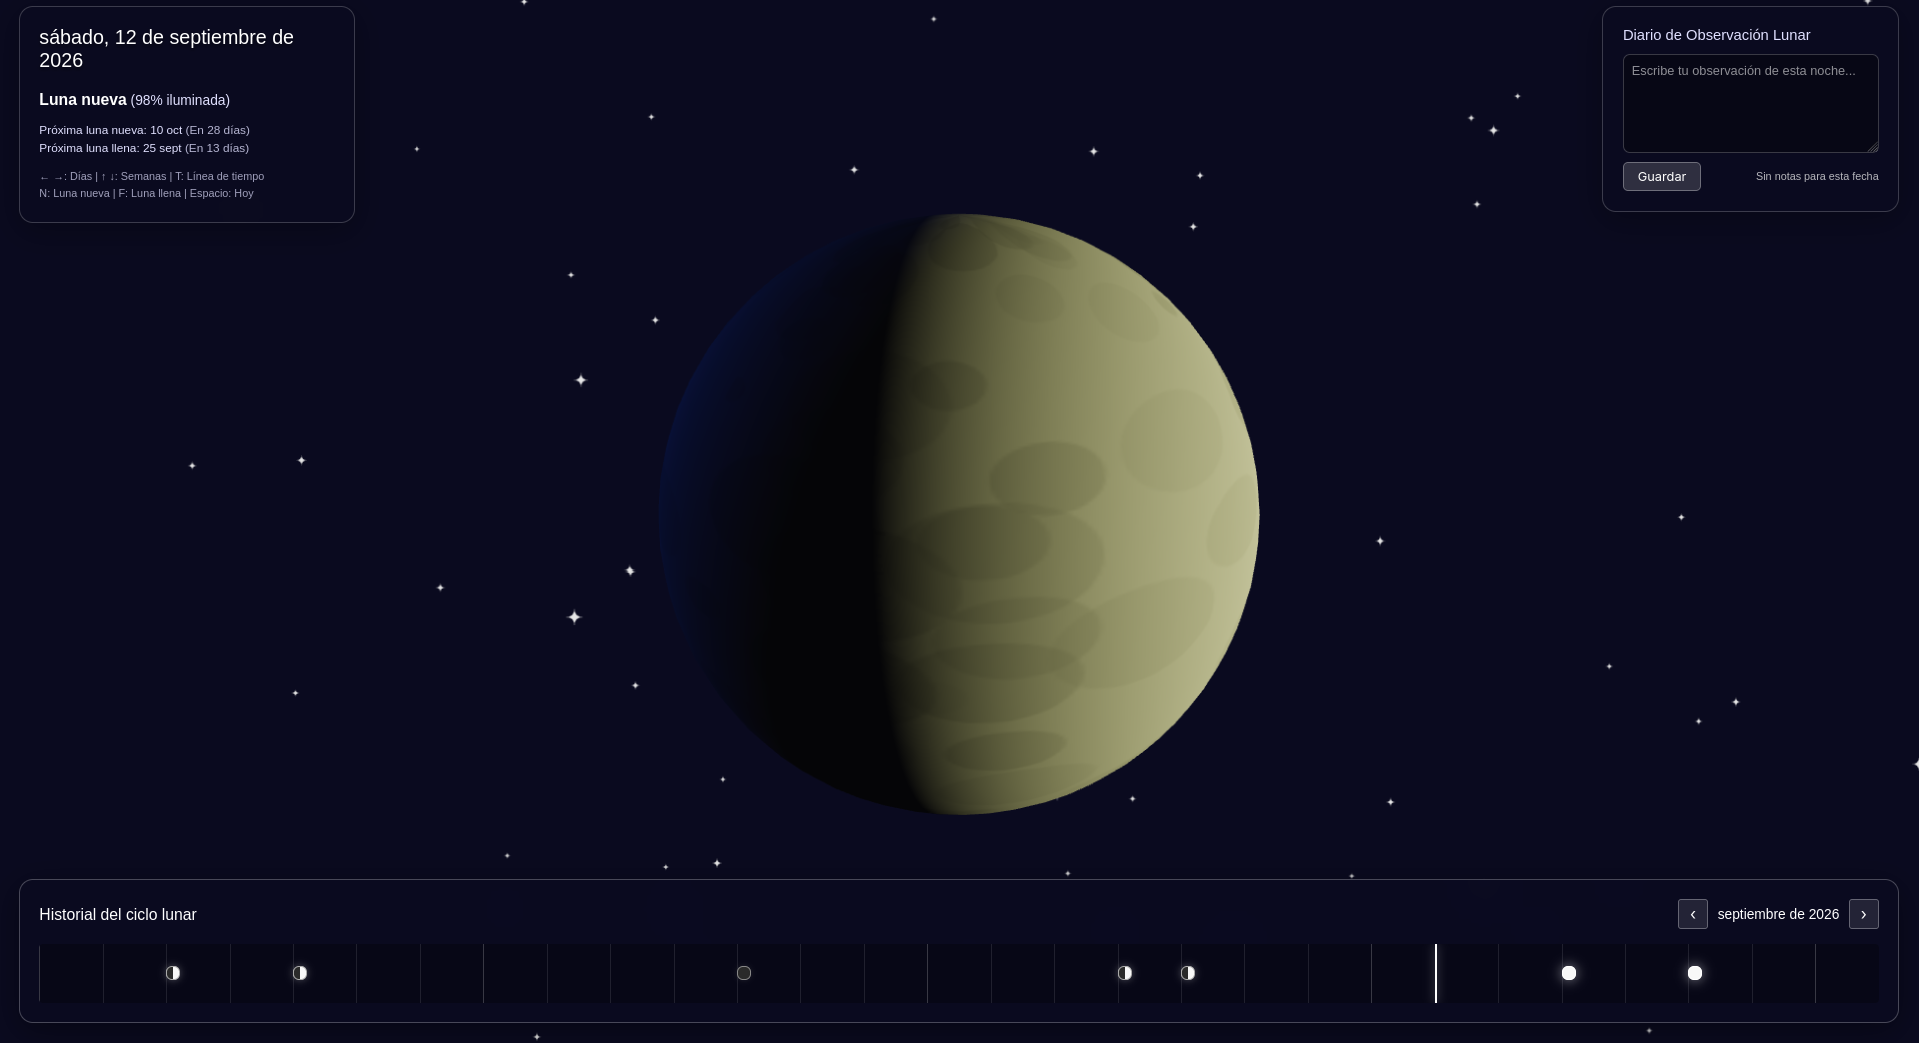
\includegraphics[width=0.92\textwidth]{content/imgs/pagina.png}
    \caption{Vista principal de la aplicación MoonPhases, con la simulación 3D del ciclo lunar y el panel de \emph{Diario de Observación Lunar}.}
\end{figure}

\subsection{Breve explicación del problema y la solución propuesta}
\emph{MoonPhases}, el proyecto original de NeaByteLab, es un simulador 3D de las fases lunares que permite recorrer el calendario y observar cómo cambia la iluminación de la luna. Sin embargo, la aplicación no permite almacenar información: el usuario no puede registrar sus observaciones ni consultarlas posteriormente.

Para resolver esta limitación, incorporamos un panel denominado \emph{Diario de Observación Lunar}, en el que el usuario puede registrar una nota asociada a una fecha y recuperarla más adelante. Para almacenar estas notas de forma persistente, reorganizamos el proyecto en tres capas:

\begin{itemize}
    \item \textbf{Frontend}: aplicación Vite + TypeScript + Three.js, servida mediante Nginx.
    \item \textbf{Backend}: API REST construida con Node.js y Express, expuesta en el puerto \texttt{3001}.
    \item \textbf{Base de datos}: PostgreSQL, con el esquema \texttt{moon\_notes} para persistir las notas.
\end{itemize}

Sobre esta base funcional, el curso de DevOps exige aplicar prácticas de control de versiones con \emph{Conventional Commits}, una metodología de \emph{branching} basada en Gitflow, y la contenerización completa de los tres servicios mediante Docker y Docker Compose, de modo que el sistema completo pueda levantarse de forma reproducible con un único comando.

\subsection{Integrantes y roles}

\begin{center}
\begin{tabularx}{\textwidth}{@{}l>{\raggedright\arraybackslash}X@{}}
\toprule
\textbf{Integrante} & \textbf{Rol dentro del proyecto} \\
\midrule
Angello Zuloaga & Adaptación del proyecto base a la arquitectura de tres capas: frontend, backend (API REST) y base de datos (esquema y conexión a PostgreSQL). \\
Eddison Pinedo & Dockerización de cada servicio (Dockerfiles, \texttt{docker-compose}), configuración de redes, volúmenes y \emph{secrets}, y documentación técnica del despliegue. \\
Nicol Campoverde & Automatización de pruebas: definición de la estrategia de pruebas unitarias y de los scripts de ejecución del proyecto. \\
\bottomrule
\end{tabularx}
\end{center}

\chapter{Justificación del proyecto}

\section{Justificación de la elección del tema}

\subsection{Contexto del proyecto}
El curso requería tomar un proyecto de software existente y aplicarle control de versiones, pruebas unitarias y contenerización. Elegimos \emph{MoonPhases} porque se trataba de una aplicación funcional compuesta únicamente por un frontend, lo que nos permitía incorporar un backend y una base de datos sin modificar su propósito original. Esta ampliación, además, generaba tareas independientes que podían distribuirse entre los tres integrantes.

En lugar de realizar un fork, creamos un repositorio nuevo, importamos el código original y lo tradujimos al español. De este modo, el historial de commits registra únicamente el trabajo del equipo desde su primer commit.

\subsection{Motivación y relevancia}
Aplicar estas prácticas sobre un proyecto real, con múltiples integrantes trabajando en paralelo sobre distintos módulos (base de datos, backend, frontend, infraestructura), permite experimentar directamente los problemas que las prácticas de DevOps buscan resolver.

Al trabajar tres integrantes sobre componentes distintos (base de datos, backend, frontend e infraestructura), era necesario un procedimiento que evitara conflictos entre los cambios de cada uno. Por ello, cada componente se desarrolló en una rama propia y se integró a \texttt{main} mediante un pull request.

Esta organización facilitó el trabajo posterior. Por ejemplo, la dockerización del backend no requirió modificar su lógica, ya que la conexión a la base de datos se configuraba mediante variables de entorno; bastó con reemplazar el host por el nombre del servicio definido en Docker Compose. Del mismo modo, el endpoint \texttt{/api/health}, creado durante el desarrollo del backend, se reutilizó para el healthcheck del contenedor.

\chapter{Control de versiones y colaboración}

\section{Aplicación de Git con Conventional Commits}

\subsection{¿Qué son los Conventional Commits y por qué se usan?}
\emph{Conventional Commits} es un estándar para redactar mensajes de commit con una estructura fija: \texttt{tipo(alcance): descripción}. El \texttt{tipo} indica la naturaleza del cambio (nueva funcionalidad, corrección, documentación, etc.) y el \texttt{alcance}, opcional, precisa el módulo afectado (por ejemplo \texttt{backend}, \texttt{frontend} o \texttt{db}).

Adoptamos esta convención porque cada integrante trabajaba sobre una capa distinta del sistema, y el alcance indicado entre paréntesis permite identificar el componente afectado por cada cambio. Por ejemplo, el mensaje \texttt{feat(backend): agregar endpoints CRUD de notas} indica, sin necesidad de revisar el código, que se trata de una nueva funcionalidad del backend.

\subsection{Tipos principales}
\begin{itemize}
  \item \texttt{feat}: nueva funcionalidad.
  \item \texttt{fix}: corrección de errores.
  \item \texttt{docs}: cambios en documentación.
  \item \texttt{test}: cambios en pruebas.
  \item \texttt{chore}: tareas de mantenimiento.
  \item \texttt{ci}: cambios en integración continua.
  \item \texttt{refactor}: refactorización sin cambiar comportamiento.
\end{itemize}

\begin{notebox}
En el historial actual del proyecto se emplearon cinco de estos tipos: \textcolor{gitfeat}{\textbf{feat}} (nueva funcionalidad de DB, backend y frontend), \textcolor{gitchore}{\textbf{chore}} (configuración de Docker y del repositorio), \textcolor{gitdocs}{\textbf{docs}} (documentación), \textcolor{gitrefactor}{\textbf{refactor}} (reorganización de carpetas) y \texttt{test} (pruebas unitarias y automatización). Los tipos \texttt{fix} y \texttt{ci} aún no se han utilizado.
\end{notebox}

\subsection{Historial de commits}

\begin{figure}[H]
    \centering
    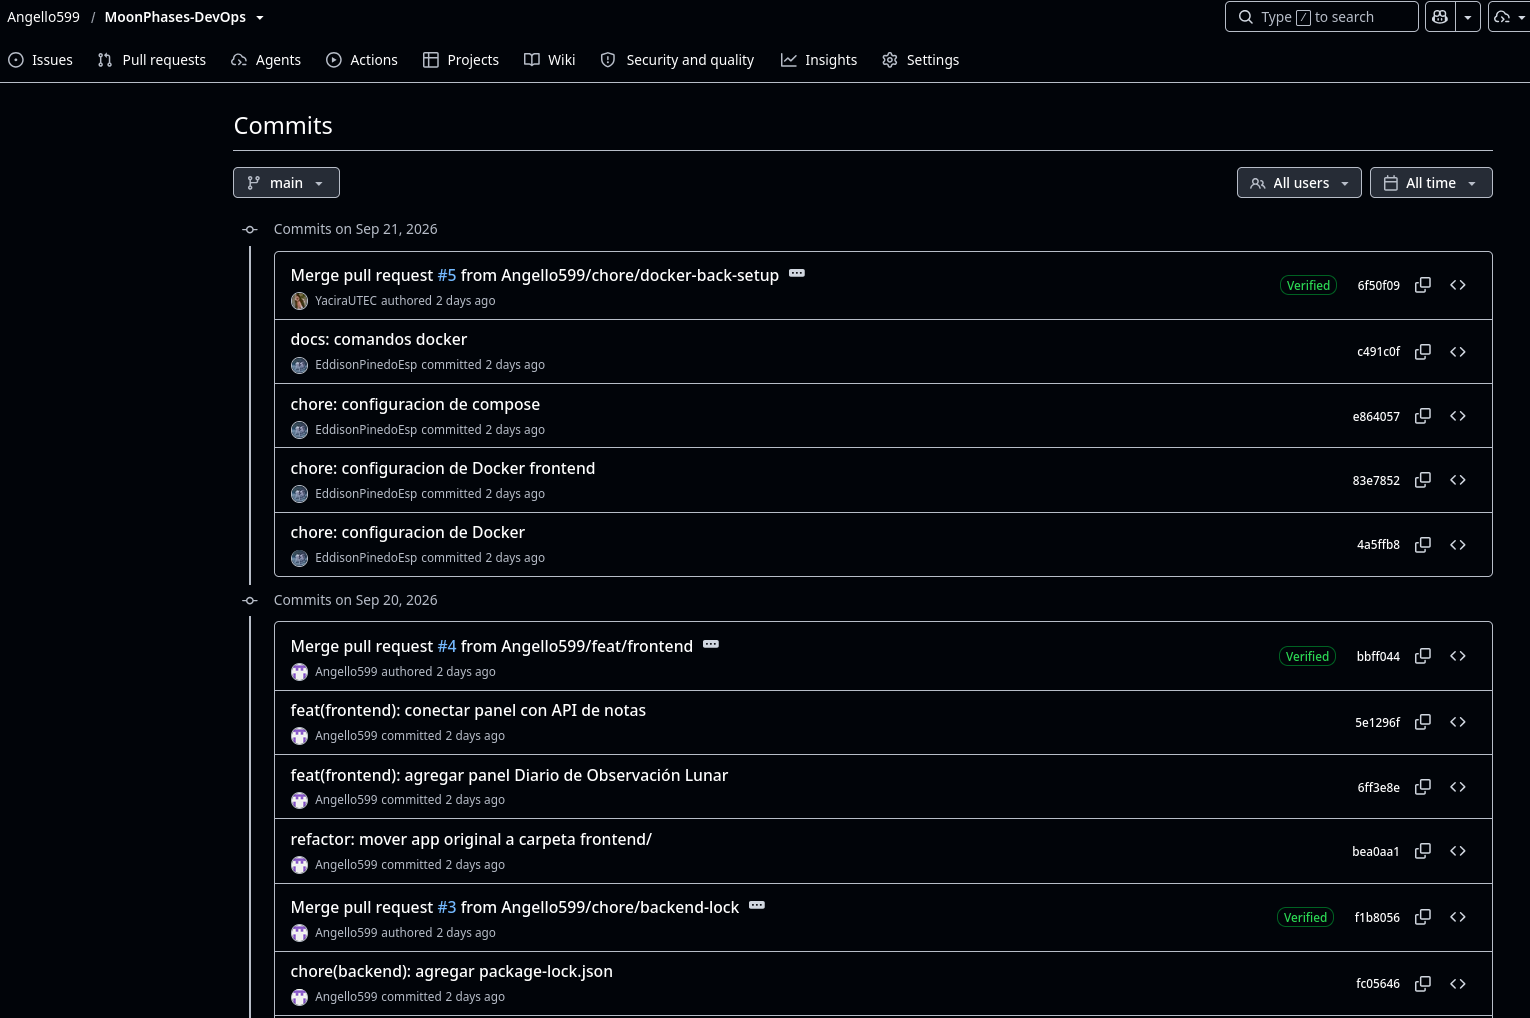
\includegraphics[width=0.92\textwidth]{content/imgs/commits.png}
    \caption{Historial de commits del repositorio \texttt{MoonPhases-DevOps} sobre la rama \texttt{main}, visualizado en GitHub.}
\end{figure}

El historial de \texttt{main} contiene 25 commits (17 commits de contenido y 8 commits de \emph{merge} de \emph{pull requests}). A continuación se analiza en detalle una muestra de 8 commits que recorre la evolución del proyecto desde la importación del código base hasta la incorporación de pruebas y su documentación.

\begin{center}
\begin{tabularx}{\textwidth}{@{}l l l >{\raggedright\arraybackslash}X@{}}
\toprule
\textbf{Hash} & \textbf{Tipo} & \textbf{Alcance} & \textbf{Mensaje y análisis} \\
\midrule

\texttt{e8c8428} &
\textcolor{gitchore}{\texttt{chore}} &
\textit{(repo)} &
\textbf{chore: importar código base de MoonPhases.}
Commit inicial que trae el proyecto original de NeaByteLab al repositorio del equipo, estableciendo el punto de partida sobre el que se construirán backend y base de datos. \\
\addlinespace

\texttt{0e24ea5} &
\textcolor{gitfeat}{\texttt{feat}} &
\texttt{db} &
\textbf{feat(db): agregar esquema de tabla moon\_notes.}
Define la tabla \texttt{moon\_notes} (fecha única, contenido, marcas de tiempo) en \texttt{backend/db/schema.sql}, la base de toda la persistencia de notas del diario lunar. \\
\addlinespace

\texttt{afeafb4} &
\textcolor{gitfeat}{\texttt{feat}} &
\texttt{backend} &
\textbf{feat(backend): agregar endpoints CRUD de notas.}
Implementa las rutas \texttt{GET/POST/DELETE} de \texttt{/api/notes} en Express, completando la API que el frontend consumirá más adelante. \\
\addlinespace

\texttt{bea0aa1} &
\textcolor{gitrefactor}{\texttt{refactor}} &
\textit{(repo)} &
\textbf{refactor: mover app original a carpeta frontend/.}
Reorganiza el repositorio monolítico en una estructura de módulos (\texttt{frontend/}, \texttt{backend/}), condición necesaria para poder dockerizar cada servicio de forma independiente. \\
\addlinespace

\texttt{6ff3e8e} &
\textcolor{gitfeat}{\texttt{feat}} &
\texttt{frontend} &
\textbf{feat(frontend): agregar panel Diario de Observación Lunar.}
Añade el componente \texttt{NotesPanel.ts}, la interfaz donde la persona usuaria escribe y consulta sus notas sobre la fase lunar. \\
\addlinespace

\texttt{c491c0f} &
\textcolor{gitdocs}{\texttt{docs}} &
\texttt{docker} &
\textbf{docs: comandos docker.}
Documenta en el \texttt{README} los comandos de \texttt{docker compose} para construir, levantar y detener el sistema, cerrando el ciclo de la primera versión dockerizada del proyecto. \\
\addlinespace

\texttt{2319035} &
\textcolor{gitrefactor}{\texttt{test}} &
\texttt{repo} &
\textbf{test: agregar pruebas unitarias y automatizacion.}
Incorpora las pruebas unitarias de la lógica astronómica y el script para ejecutarlas, estableciendo una primera base de validación automática del proyecto. \\
\addlinespace

\texttt{ba66095} &
\textcolor{gitdocs}{\texttt{docs}} &
\texttt{repo} &
\textbf{docs: documentar ejecucion de pruebas.}
Amplía la documentación del proyecto con las instrucciones para ejecutar la suite de pruebas, haciendo reproducible la verificación de la aplicación. \\

\bottomrule
\end{tabularx}
\end{center}



\subsection{Pull requests según su metodología de branching}

La metodología de \emph{branching} utilizada es \textbf{Gitflow}: ninguna persona del equipo trabaja directamente sobre \texttt{main}. Cada tarea (una capa del sistema o una tarea de infraestructura) se desarrolla en una rama de corta duración nombrada \texttt{tipo/alcance} (por ejemplo \texttt{feat/backend} o \texttt{chore/docker-back-setup}), que se integra a \texttt{main} exclusivamente a través de un \emph{pull request} revisado en GitHub. \texttt{main} actúa así como la rama estable e íntegra en todo momento, y cada \emph{merge} queda registrado como un commit propio, lo que preserva en el grafo el contexto de en qué rama y bajo qué \emph{pull request} se hizo cada grupo de cambios.

\begin{center}
\begin{tabularx}{\textwidth}{@{}c l l >{\raggedright\arraybackslash}X@{}}
\toprule
\textbf{PR} & \textbf{Rama} & \textbf{Tipo} & \textbf{Descripción} \\
\midrule
\#1 & \texttt{feat/db} & \textcolor{gitfeat}{feature} & Esquema de la tabla \texttt{moon\_notes} y configuración de la conexión a PostgreSQL mediante variables de entorno. \\
\#2 & \texttt{feat/backend} & \textcolor{gitfeat}{feature} & Inicialización del servidor Express y endpoints CRUD de \texttt{/api/notes}. \\
\#3 & \texttt{chore/backend-lock} & \textcolor{gitchore}{chore} & Incorporación de \texttt{package-lock.json} para fijar versiones de dependencias del backend. \\
\#4 & \texttt{feat/frontend} & \textcolor{gitfeat}{feature} & Migración del proyecto original a \texttt{frontend/} y conexión del panel de notas con la API del backend. \\
\#6 & \texttt{feature/testing} & \textcolor{gitfeat}{feature} & Incorporación de pruebas unitarias para la lógica astronómica y automatización de su ejecución con Vitest. \\
\bottomrule
\end{tabularx}
\end{center}

\begin{figure}[H]
    \centering
    \resizebox{\textwidth}{!}{%
    \begin{tikzpicture}[
        x=1cm, y=1cm,
        commitdot/.style={
            circle,
            draw=reportdark,
            fill=#1,
            minimum size=7pt,
            inner sep=0pt,
            line width=0.5pt
        },
        mergedot/.style={
            diamond,
            draw=reportdark,
            fill=gitmerge,
            minimum size=10pt,
            inner sep=0pt,
            line width=0.5pt
        },
        mainline/.style={
            reportdark,
            line width=1.1pt
        },
        developline/.style={
            reportblue,
            line width=1.0pt
        },
        branchline/.style={
            reportgray,
            line width=0.8pt
        },
        branchlabel/.style={
            font=\tiny\ttfamily,
            reportgray,
            anchor=south
        },
        prlabel/.style={
            font=\scriptsize\sffamily\bfseries,
            reportblue,
            anchor=south
        },
        devlabel/.style={
            font=\bfseries\sffamily\small,
            reportblue
        }
    ]

        % =========================================================
        % MAIN
        % =========================================================
        \draw[mainline] (-0.5,0) -- (15.5,0);

        \node[
            anchor=east,
            font=\bfseries\sffamily\small,
            reportdark
        ] at (-0.6,0) {main};

        % Commits iniciales
        \node[commitdot=gitchore] (c1) at (0,0) {};
        \node[commitdot=gitdocs]  (c2) at (0.7,0) {};
        \node[commitdot=gitchore] (c3) at (1.4,0) {};

        % =========================================================
        % DEVELOP
        % =========================================================
        \draw[developline]
            (1.4,0)
            .. controls +(0.15,0.7) and +(-0.15,0.7) ..
            (1.8,2.0)
            -- (15.0,2.0);

        \node[
            anchor=east,
            devlabel
        ] at (1.55,2.0) {develop};

        % Commit inicial de develop
        \node[commitdot=gitchore] at (1.8,2.0) {};

        % =========================================================
        % PR #1 - feat/db
        % =========================================================
        \draw[branchline]
            (2.0,2.0)
            .. controls +(0.15,0.65) and +(-0.15,0.65) ..
            (2.35,3.15)
            -- (3.05,3.15)
            .. controls +(0.15,-0.65) and +(-0.15,-0.65) ..
            (3.4,2.0);

        \node[commitdot=gitfeat] at (2.35,3.15) {};
        \node[commitdot=gitfeat] at (3.05,3.15) {};

        \node[branchlabel] at (2.7,3.4) {feat/db};

        \node[mergedot] at (3.4,2.0) {};

        % =========================================================
        % PR #2 - feat/backend
        % =========================================================
        \draw[branchline]
            (3.6,2.0)
            .. controls +(0.15,0.65) and +(-0.15,0.65) ..
            (4.0,3.15)
            -- (4.8,3.15)
            .. controls +(0.15,-0.65) and +(-0.15,-0.65) ..
            (5.2,2.0);

        \node[commitdot=gitfeat] at (4.0,3.15) {};
        \node[commitdot=gitfeat] at (4.8,3.15) {};

        \node[branchlabel] at (4.4,3.4) {feat/backend};

        \node[mergedot] at (5.2,2.0) {};

        % =========================================================
        % PR #3 - chore/backend-lock
        % =========================================================
        \draw[branchline]
            (5.4,2.0)
            .. controls +(0.2,0.65) and +(-0.2,0.65) ..
            (6.4,3.15)
            .. controls +(0.2,-0.65) and +(-0.2,-0.65) ..
            (7.4,2.0);

        \node[commitdot=gitchore] at (6.4,3.15) {};

        \node[branchlabel] at (6.4,3.4) {chore/backend-lock};

        \node[mergedot] at (7.4,2.0) {};

        % =========================================================
        % PR #4 - feat/frontend
        % =========================================================
        \draw[branchline]
            (7.6,2.0)
            .. controls +(0.15,0.65) and +(-0.15,0.65) ..
            (8.0,3.15)
            -- (9.3,3.15)
            .. controls +(0.15,-0.65) and +(-0.15,-0.65) ..
            (9.7,2.0);

        \node[commitdot=gitrefactor] at (8.0,3.15) {};
        \node[commitdot=gitfeat]     at (8.65,3.15) {};
        \node[commitdot=gitfeat]     at (9.3,3.15) {};

        \node[branchlabel] at (8.65,3.4) {feat/frontend};

        \node[mergedot] at (9.7,2.0) {};

        % =========================================================
        % PR #5 - develop -> main
        % Integración de las primeras features
        % =========================================================
        \draw[branchline]
            (9.9,2.0)
            .. controls +(0.15,-0.65) and +(-0.15,-0.65) ..
            (10.3,0);

        \node[mergedot] at (10.3,0) {};

        % =========================================================
        % CHORE/DOCKER-BACK-SETUP
        % Sale de develop
        % =========================================================
        \draw[branchline]
            (10.0,2.0)
            .. controls +(0.2,0.65) and +(-0.2,0.65) ..
            (10.5,3.15)
            -- (12.7,3.15)
            .. controls +(0.2,-0.65) and +(-0.2,-0.65) ..
            (13.2,2.0);

        \node[commitdot=gitchore] at (10.5,3.15) {};
        \node[commitdot=gitchore] at (11.25,3.15) {};
        \node[commitdot=gitchore] at (12.0,3.15) {};
        \node[commitdot=gitdocs]  at (12.7,3.15) {};

        \node[branchlabel] at (11.6,3.4)
            {chore/docker-back-setup};

        \node[mergedot] at (13.2,2.0) {};

        % =========================================================
        % PR #7 - develop -> main
        % Docker integrado
        % =========================================================
        \draw[branchline]
            (13.4,2.0)
            .. controls +(0.15,-0.65) and +(-0.15,-0.65) ..
            (13.8,0);

        \node[mergedot] at (13.8,0) {};

        % =========================================================
        % TEST: PRUEBAS UNITARIAS
        % Sale de develop y retorna a develop
        % =========================================================
        \draw[branchline]
            (13.5,2.0)
            .. controls +(0.15,0.65) and +(-0.15,0.65) ..
            (14.0,3.15)
            -- (14.9,3.15)
            .. controls +(0.15,-0.65) and +(-0.15,-0.65) ..
            (15.2,2.0);
        
        \node[commitdot=gitfix] at (14.0,3.15) {};
        \node[commitdot=gitfix] at (14.45,3.15) {};
        \node[commitdot=gitfix] at (14.9,3.15) {};
        
        \node[branchlabel] at (14.45,3.4)
            {test/unitarias};
        
        \node[mergedot] at (15.2,2.0) {};

        % =========================================================
        % PR #9 - develop -> main
        % Integración final de pruebas
        % =========================================================
        \draw[branchline]
            (15.0,2.0)
            .. controls +(0.15,-0.65) and +(-0.15,-0.65) ..
            (15.5,0);

        \node[mergedot] at (15.5,0) {};

        % =========================================================
        % Leyenda
        % =========================================================
        \begin{scope}[
            shift={(-0.5,-1.7)},
            font=\small\sffamily
        ]
            \node[
                commitdot=gitfeat,
                label=right:{feat}
            ] at (0,0) {};

            \node[
                commitdot=gitfix,
                label=right:{fix / test}
            ] at (2.1,0) {};

            \node[
                commitdot=gitdocs,
                label=right:{docs}
            ] at (4.2,0) {};

            \node[
                commitdot=gitchore,
                label=right:{chore}
            ] at (6.3,0) {};

            \node[
                commitdot=gitrefactor,
                label=right:{refactor}
            ] at (8.4,0) {};

            \node[
                mergedot,
                label=right:{merge}
            ] at (10.7,0) {};
        \end{scope}

    \end{tikzpicture}%
    }
    \caption{
        Flujo de trabajo basado en Gitflow. Las ramas de funcionalidades
        (\texttt{feat}) y tareas (\texttt{chore}) se crean a partir de
        \texttt{develop} y se integran mediante \emph{pull requests}.
        Posteriormente, los cambios acumulados en \texttt{develop} se
        integran en \texttt{main}. La rama de pruebas unitarias sigue el
        mismo flujo de integración antes de la publicación final.
    }
\end{figure}


\chapter{Pruebas unitarias}

\section{Implementación de pruebas unitarias}
\subsection{Herramienta utilizada}
La herramienta que se utilizó para realizar las pruebas es \texttt{Vitest}.

\subsection{Implementación de test}

Se implementaron nueve pruebas unitarias utilizando \textbf{Vitest}, con el objetivo de verificar el comportamiento de las principales funciones de cálculo y procesamiento de fechas relacionadas con las fases lunares. Las pruebas se encuentran organizadas en el archivo \texttt{tests/ta.test.ts} y evalúan funciones del módulo \texttt{frontend/src/core/ta.ts}.

Las pruebas implementadas son las siguientes:

\begin{enumerate}
    \item \textbf{Validación de una fecha válida:} se verifica que la función \texttt{validateDate()} acepte correctamente una fecha válida sin generar una excepción.

    \item \textbf{Validación de una fecha inválida:} se comprueba que \texttt{validateDate()} genere una excepción cuando recibe un valor de fecha no válido.

    \item \textbf{Cálculo del día juliano:} se verifica que la función \texttt{julianDay()} obtenga correctamente el día juliano para una fecha de referencia. Para el caso utilizado en la prueba, el resultado esperado es aproximadamente \(2451545.0\).

    \item \textbf{Cálculo de la fase lunar:} se comprueba que \texttt{moonPhase()} devuelva un valor dentro del intervalo válido de \(0\) a \(1\), correspondiente a la representación de la fase lunar.

    \item \textbf{Identificación de Luna nueva:} se verifica que \texttt{phaseName()} identifique correctamente el valor de fase \(0\) como ``Luna nueva''.

    \item \textbf{Identificación de Luna llena:} se comprueba que \texttt{phaseName()} identifique correctamente el valor de fase \(0.5\) como ``Luna llena''.

    \item \textbf{Cálculo de iluminación:} se verifica que \texttt{illumination()} obtenga aproximadamente un \(100\% \) de iluminación para una fase de \(0\).

    \item \textbf{Diferencia entre fechas:} se comprueba que \texttt{daysBetween()} calcule correctamente la cantidad de días entre dos fechas. Para las fechas utilizadas en la prueba, el resultado esperado es de 9 días.

    \item \textbf{Formato de tiempo relativo:} se verifica que \texttt{formatRelativeTime()} devuelva ``Hoy'' cuando recibe un valor de cero días.
\end{enumerate}

La ejecución de estas pruebas se realiza desde la raíz del proyecto mediante el comando:

\begin{lstlisting}
npm test
\end{lstlisting}


\newpage
\subsection{Evidencia de ejecución de los tests}

Pruebas unitarias
\begin{figure}[H]
    \centering
    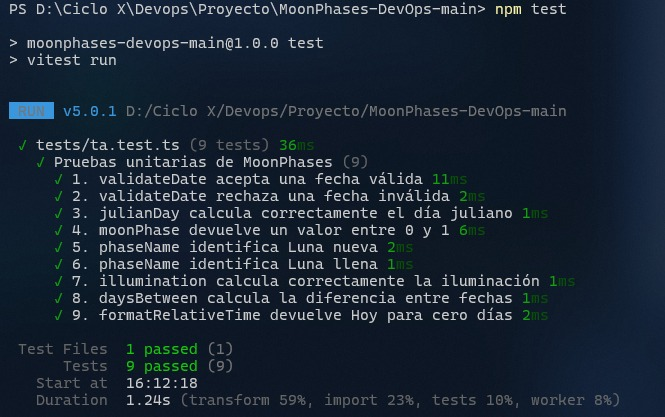
\includegraphics[width=0.80\textwidth]{content/imgs/k1.jpeg}
    \caption{Pruebas unitarias de MoonPhases.}
\end{figure}

\chapter{Automatización de tareas}

\section{Automatización en scripts bash}
\subsection{Automatizar la clonación del proyecto}

Para automatizar la obtención del código fuente del proyecto se implementó
el script \texttt{clone-project.sh}, ubicado en la raíz del repositorio.
Este script permite clonar automáticamente el repositorio de MoonPhases
sin necesidad de ejecutar manualmente el comando de clonación.

El contenido del script es el siguiente:

\begin{lstlisting}[language=bash]
#!/bin/bash

REPO_URL="https://github.com/Angello599/MoonPhases-DevOps.git"
PROJECT_DIR="MoonPhases-DevOps"

echo "======================================"
echo "   CLONANDO PROYECTO MOONPHASES"
echo "======================================"

if [ -d "$PROJECT_DIR" ]; then
    echo "El directorio $PROJECT_DIR ya existe."
    exit 1
fi

git clone "$REPO_URL" "$PROJECT_DIR"

if [ $? -eq 0 ]; then
    echo ""
    echo "======================================"
    echo "   PROYECTO CLONADO CORRECTAMENTE"
    echo "======================================"
else
    echo ""
    echo "======================================"
    echo "   ERROR AL CLONAR EL PROYECTO"
    echo "======================================"
    exit 1
fi
\end{lstlisting}

El script define la URL del repositorio y el nombre del directorio donde se
almacenará el proyecto. Antes de realizar la clonación, verifica si el
directorio de destino ya existe para evitar sobrescribir una copia
existente. Si el directorio no existe, ejecuta \texttt{git clone} para
descargar el repositorio. Finalmente, verifica el código de salida de la
operación e informa si la clonación se realizó correctamente o si ocurrió
un error.

Para ejecutar el script se utiliza el siguiente comando desde Git Bash:

\begin{lstlisting}[language=bash]
./clone-project.sh
\end{lstlisting}

De esta manera, la clonación del repositorio queda automatizada mediante un
script Bash y puede ejecutarse utilizando un único comando.

\begin{figure}[H]
    \centering
    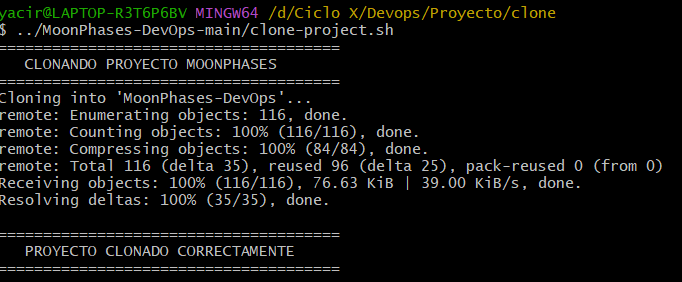
\includegraphics[width=0.80\textwidth]{content/imgs/k3.png}
    \caption{Automatización de clonación del proyecto.}
\end{figure}

\subsection{Automatizar la ejecución de los test}

Para automatizar la ejecución de las pruebas unitarias se implementó el
script \texttt{run-tests.sh}, ubicado en la raíz del repositorio. Este
script permite ejecutar las pruebas mediante un único comando y verificar
automáticamente si fueron ejecutadas correctamente.

El contenido del script es el siguiente:

\begin{lstlisting}[language=bash]
#!/bin/bash

echo "======================================"
echo "   EJECUTANDO TESTS DE MOONPHASES"
echo "======================================"

npm test

if [ $? -eq 0 ]; then
    echo ""
    echo "======================================"
    echo "   TODOS LOS TESTS PASARON"
    echo "======================================"
else
    echo ""
    echo "======================================"
    echo "   ALGUN TEST FALLO"
    echo "======================================"
    exit 1
fi
\end{lstlisting}

El script ejecuta el comando \texttt{npm test}, que inicia Vitest y ejecuta
las nueve pruebas unitarias implementadas. Posteriormente, se verifica el
código de salida del proceso. Si el resultado es exitoso, se muestra un
mensaje indicando que todas las pruebas pasaron. En caso contrario, el
script informa que alguna prueba falló y finaliza con código de error.

Para ejecutar la automatización se utiliza:

\begin{lstlisting}[language=bash]
./run-tests.sh
\end{lstlisting}

El archivo se encuentra directamente en la raíz del proyecto, permitiendo
que la ejecución de las pruebas sea reproducible sin necesidad de ejecutar
cada prueba individualmente.

\begin{figure}[H]
    \centering
    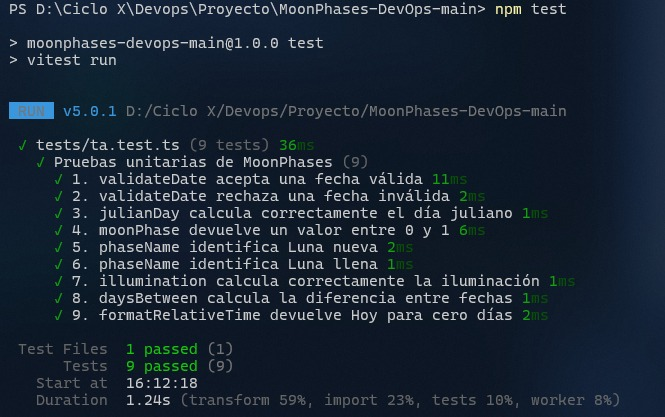
\includegraphics[width=0.80\textwidth]{content/imgs/k1.jpeg}
    \caption{Automatización de ejecución de test.}
\end{figure}


\subsection{Automatizar correr el proyecto en modo local}

Para automatizar el levantamiento del proyecto en modo local se implementó
el script \texttt{run-local.sh}, ubicado en la raíz del repositorio. Este
script permite iniciar los servicios de MoonPhases mediante Docker Compose
sin necesidad de ejecutar manualmente los comandos correspondientes.

El contenido del script es el siguiente:

\begin{lstlisting}[language=bash]
#!/bin/bash

echo "======================================"
echo "   LEVANTANDO MOONPHASES EN LOCAL"
echo "======================================"

if ! command -v docker &> /dev/null
then
    echo "ERROR: Docker no está instalado o no está disponible."
    exit 1
fi

docker compose up --build -d

if [ $? -eq 0 ]; then
    echo ""
    echo "======================================"
    echo "   MOONPHASES SE EJECUTA EN LOCAL"
    echo "======================================"
    echo ""
    echo "Frontend:"
    echo "http://localhost:8080/MoonPhases/"
    echo ""
    echo "Backend:"
    echo "http://localhost:3001/api/health"
else
    echo ""
    echo "======================================"
    echo "   ERROR AL LEVANTAR EL PROYECTO"
    echo "======================================"
    exit 1
fi
\end{lstlisting}

El script verifica inicialmente que Docker se encuentre disponible. Luego
ejecuta el comando \texttt{docker compose up --build -d}, mediante el cual
se construyen las imágenes necesarias y se levantan los servicios definidos
en el archivo \texttt{compose.yaml} en segundo plano.

Para ejecutar el script se utiliza el siguiente comando desde la raíz del
proyecto:

\begin{lstlisting}[language=bash]
./run-local.sh
\end{lstlisting}

\begin{figure}[H]
    \centering
    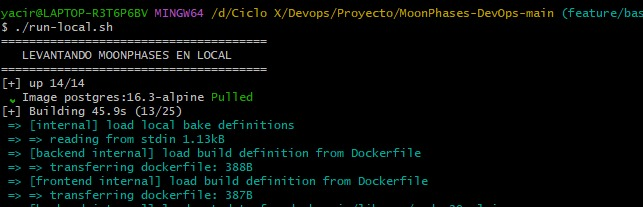
\includegraphics[width=0.9\textwidth]{content/imgs/run-loca.jpg}
        \caption{Automatización para correr el proyecto local.}
\end{figure}
\chapter{Contenerización de la aplicación}

\section{Configuración de Docker}

\subsection{Dockerfiles y Docker Compose}
Cada servicio de MoonPhases tiene su propio \texttt{Dockerfile}, y \texttt{compose.yaml} en la raíz del repositorio orquesta los tres contenedores (frontend, backend y base de datos) junto con sus redes, volúmenes y \emph{secrets}.

\textbf{Backend (\texttt{backend/Dockerfile}).} Imagen basada en \texttt{node:20-alpine}. Instala únicamente dependencias de producción (\texttt{npm ci --omit=dev}), copia el código fuente con propietario \texttt{node} y ejecuta el proceso como usuario no privilegiado (\texttt{USER node}), en vez de \texttt{root}. Declara un \texttt{HEALTHCHECK} que consulta \texttt{/api/health} cada 15 segundos, información que Compose usa para decidir cuándo el servicio está realmente disponible.

\textbf{Frontend (\texttt{frontend/Dockerfile}).} Usa una \emph{build} de dos etapas: la primera etapa (\texttt{node:20-alpine}) instala dependencias y ejecuta \texttt{vite build}, generando los archivos estáticos optimizados; la segunda etapa parte de \texttt{nginx-unprivileged:alpine} y copia únicamente el resultado de la compilación (\texttt{/app/dist}) junto con la configuración de \texttt{nginx.conf}. El contenedor final no contiene Node.js, \texttt{node\_modules} ni código fuente, sólo los estáticos y Nginx corriendo sin privilegios de \texttt{root}.

\textbf{Base de datos.} No se construye una imagen propia: se usa directamente \texttt{postgres:16.3-alpine}, inicializada con \texttt{backend/db/schema.sql} montado en \texttt{/docker-entrypoint-initdb.d/}, de modo que la tabla \texttt{moon\_notes} se crea automáticamente la primera vez que se crea el volumen de datos.

El contenido de los archivos de construcción es el siguiente:

\textbf{\texttt{backend/Dockerfile}}
\begin{lstlisting}[language=bash]
FROM node:20-alpine

WORKDIR /app
ENV NODE_ENV=production

COPY package*.json ./
RUN npm ci --omit=dev && npm cache clean --force

COPY --chown=node:node src ./src

USER node
EXPOSE 3001

HEALTHCHECK --interval=15s --timeout=5s --retries=3 \
    CMD wget -qO- http://localhost:3001/api/health || exit 1

CMD ["node", "src/server.js"]
\end{lstlisting}

\textbf{\texttt{frontend/Dockerfile}}
\begin{lstlisting}[language=bash]
FROM node:20-alpine AS build

WORKDIR /app

COPY package*.json ./
RUN npm ci

COPY vite.config.ts tsconfig.json ./
COPY index.html ./
COPY src ./src
RUN npm run build

FROM nginxinc/nginx-unprivileged:alpine

COPY nginx.conf /etc/nginx/conf.d/default.conf
COPY --from=build /app/dist /usr/share/nginx/html/MoonPhases

EXPOSE 8080
\end{lstlisting}

\textbf{\texttt{compose.yaml}}
\begin{lstlisting}[language=yaml]
services:
    postgres:
        image: postgres:16.3-alpine
        restart: unless-stopped
        environment:
            - POSTGRES_USER=moonuser
            - POSTGRES_DB=moonphases_db
            - POSTGRES_PASSWORD_FILE=/run/secrets/pg_password
        secrets:
            - pg_password
        volumes:
            - postgres-data:/var/lib/postgresql/data
            - ./backend/db/schema.sql:/docker-entrypoint-initdb.d/schema.sql:ro
        networks:
            - private
        healthcheck:
            test: ["CMD-SHELL", "pg_isready -U moonuser -d moonphases_db"]
            interval: 5s
            timeout: 5s
            retries: 5

    backend:
        build: ./backend
        image: moonphases-backend:1.0.0
        restart: unless-stopped
        ports:
            - "3001:3001"
        environment:
            - PORT=3001
            - DB_HOST=postgres
            - DB_PORT=5432
            - DB_USER=moonuser
            - DB_NAME=moonphases_db
            - DB_PASSWORD_FILE=/run/secrets/pg_password
        secrets:
            - pg_password
        networks:
            - public
            - private
        depends_on:
            postgres:
                condition: service_healthy

    frontend:
        build: ./frontend
        image: moonphases-frontend:1.0.0
        restart: unless-stopped
        ports:
            - "8080:8080"
        networks:
            - public
        depends_on:
            - backend

secrets:
    pg_password:
        file: ./pg_password.txt

volumes:
    postgres-data:

networks:
    public:
    private:
        internal: true
\end{lstlisting}

\begin{figure}[H]
    \centering
    \resizebox{0.92\textwidth}{!}{%
    \begin{tikzpicture}[
        stage/.style={draw=reportdark, thick, rounded corners=2mm, minimum width=3.1cm, minimum height=1.5cm, align=center, font=\small\sffamily},
        artifact/.style={draw=dockvolume, thick, rounded corners=1mm, fill=white, minimum width=2.2cm, minimum height=0.9cm, align=center, font=\scriptsize\sffamily},
        arrowstyle/.style={-{Stealth[length=2.2mm]}, reportgray, thick}
        ]
        \node[stage, fill=reportbg] (s1) at (0,0) {\textbf{Etapa 1: build}\\[2pt] \texttt{node:20-alpine}\\[2pt] \footnotesize \texttt{npm ci}\\\texttt{vite build}};
        \node[artifact] (art) at (5.4,0) {\texttt{/app/dist}\\[1pt]\footnotesize estáticos optimizados};
        \node[stage, fill=reportbg] (s2) at (10.8,0) {\textbf{Etapa 2: runtime}\\[2pt] \texttt{nginx-unprivileged}\\[2pt]\footnotesize \texttt{:alpine} (usuario no root)};

        \draw[arrowstyle] (s1) -- (art) node[midway, above=2pt, font=\scriptsize\sffamily, gitmerge] {\texttt{COPY --from=build}};
        \draw[arrowstyle] (art) -- (s2);

        \node[font=\scriptsize\sffamily, reportgray, below=2pt of s1] {no viaja al contenedor final};
        \node[font=\scriptsize\sffamily, gitfeat, below=2pt of s2] {imagen final: 8080/tcp};
    \end{tikzpicture}%
    }
    \caption{Construcción \emph{multi-stage} del frontend: la imagen final sólo conserva los estáticos generados por Vite y Nginx, sin herramientas de compilación.}
\end{figure}

\subsection{Ejemplo del servicio web y base de datos}
La topología completa se define en \texttt{compose.yaml}, que conecta los tres servicios mediante dos redes con propósitos distintos, siguiendo el principio de menor privilegio:

\begin{itemize}
    \item \textbf{Red \texttt{public}}: expone \texttt{frontend} (puerto \texttt{8080}) y \texttt{backend} (puerto \texttt{3001}) al host.
    \item \textbf{Red \texttt{private} (\texttt{internal: true})}: sólo conecta \texttt{backend} con \texttt{postgres}; al ser interna, PostgreSQL no tiene salida ni entrada directa desde fuera de los contenedores.
    \item \textbf{Secret \texttt{pg\_password}}: la contraseña de la base de datos se monta como archivo en \texttt{/run/secrets/pg\_password} en vez de pasarse como variable de entorno en texto plano, y la leen tanto \texttt{postgres} (\texttt{POSTGRES\_PASSWORD\_FILE}) como el backend (\texttt{DB\_PASSWORD\_FILE}, leído en \texttt{db.js}).
    \item \textbf{Volumen \texttt{postgres-data}}: persiste los datos de PostgreSQL fuera del ciclo de vida del contenedor.
    \item \textbf{\texttt{depends\_on} con \texttt{condition: service\_healthy}}: el backend no arranca hasta que el \texttt{healthcheck} de PostgreSQL (\texttt{pg\_isready}) reporte éxito.
\end{itemize}

\begin{figure}[H]
    \centering
    \begin{tikzpicture}[
        container/.style={draw=reportdark, thick, rounded corners=2mm, fill=white, minimum width=2.7cm, minimum height=1.3cm, align=center, font=\small\sffamily},
        netbox/.style={draw, thick, rounded corners=2mm, inner sep=10pt, dashed},
        vol/.style={draw=dockvolume, thick, rounded corners=1mm, fill=white, minimum width=2.3cm, minimum height=0.8cm, align=center, font=\scriptsize\sffamily},
        arrowstyle/.style={-{Stealth[length=2mm]}, reportgray, thick}
        ]

        \node[container] (fe) at (0,3.3) {\textbf{frontend}\\ \footnotesize nginx-unprivileged\\ :8080};
        \node[container] (be) at (0,0) {\textbf{backend}\\ \footnotesize node + express\\ :3001};
        \node[container] (db) at (0,-3.3) {\textbf{postgres}\\ \footnotesize postgres:16.3-alpine\\ :5432};

        \node[netbox, draw=netpublic, fit={(fe) (be)}, label={[font=\scriptsize\sffamily\bfseries, netpublic]above:red \texttt{public}}] (netpub) {};
        \node[netbox, draw=netprivate, fit={(be) (db)}, label={[font=\scriptsize\sffamily\bfseries, netprivate, xshift=1.1cm]below:red \texttt{private} (\texttt{internal: true})}] (netpriv) {};

        \node[vol, right=1.6cm of db] (vol) {\texttt{postgres-data}\\ \footnotesize volumen};
        \node[vol, right=1.6cm of be] (sec) {\texttt{pg\_password}\\ \footnotesize secret};

        \node[right=2.6cm of fe, font=\scriptsize\sffamily, reportgray, align=left] (host) {host\\ \texttt{localhost:8080}};

        \draw[arrowstyle] (fe) -- node[midway, right, font=\scriptsize\ttfamily] {/api/*} (be);
        \draw[arrowstyle] (be) -- (db);
        \draw[arrowstyle] (db) -- (vol);
        \draw[arrowstyle] (be) -- (sec);
        \draw[arrowstyle, netpublic] (host) -- (fe);

    \end{tikzpicture}
    \caption{Topología de \texttt{compose.yaml}: la red \textcolor{netpublic}{\textbf{public}} expone frontend y backend al host; la red \textcolor{netprivate}{\textbf{private}} aísla a PostgreSQL, accesible únicamente desde el backend. El volumen persiste los datos y el \emph{secret} evita contraseñas en texto plano.}
\end{figure}

Nginx además actúa como \emph{reverse proxy} interno: cualquier petición a \texttt{/api/} recibida por el contenedor \texttt{frontend} se reenvía a \texttt{http://backend:3001} usando el nombre de servicio de Compose como resolución DNS interna (ver \texttt{nginx.conf}), por lo que el navegador sólo necesita conocer el puerto \texttt{8080}.

\subsection{Evidencia de ejecución en Docker}
Con el sistema levantado mediante \texttt{docker compose up --build -d}, se verificó el estado de los tres servicios y la comunicación entre ellos.

\begin{figure}[H]
    \centering
    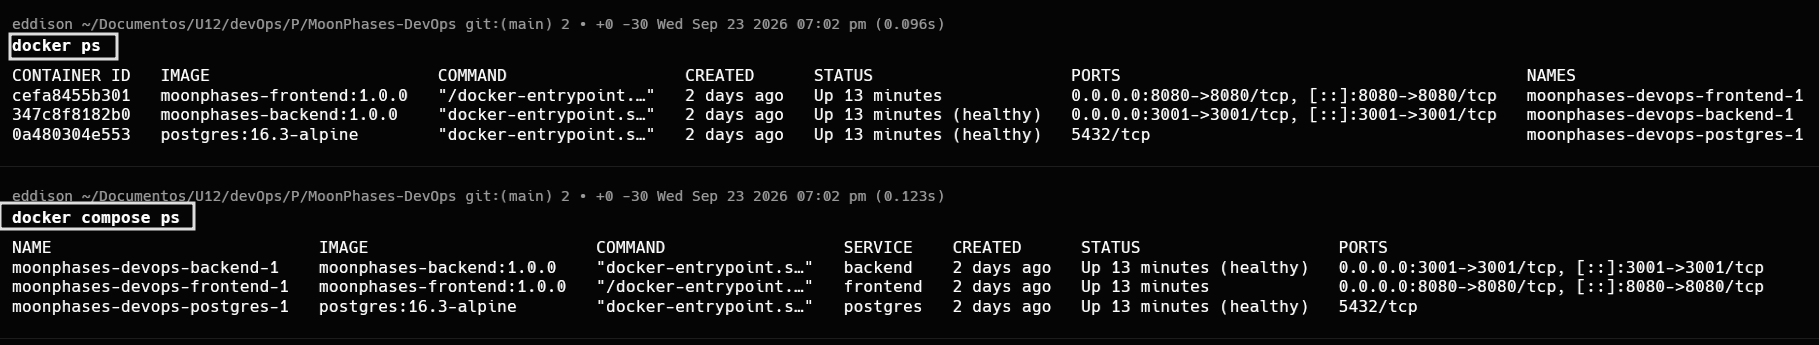
\includegraphics[width=1 \textwidth]{content/imgs/docker_ps.png}
\end{figure}

\begin{figure}[H]
    \centering
    
\includegraphics[width=1 \textwidth]{content/imgs/curl_h.png}
\end{figure}

\begin{figure}[H]
    \centering
    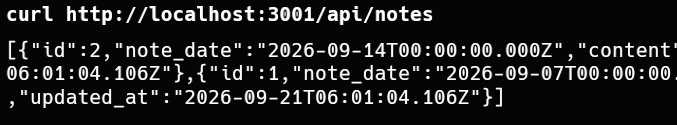
\includegraphics[width=1 \textwidth]{content/imgs/curl_notes.png}
\end{figure}

\begin{figure}[H]
    \centering
    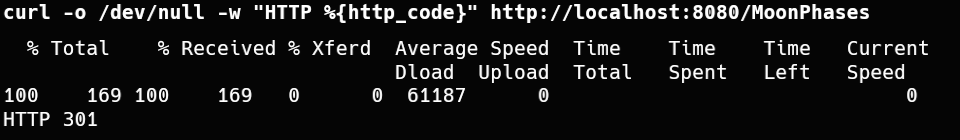
\includegraphics[width=1 \textwidth]{content/imgs/curl_code.png}
\end{figure}


Estas cuatro comprobaciones confirman, en orden, que: (1) los tres contenedores están en ejecución y los que tienen \texttt{healthcheck} reportan estado saludable; (2) el backend responde directamente en el puerto publicado \texttt{3001}; (3) el backend consulta correctamente PostgreSQL a través de la red privada y devuelve las notas sembradas por \texttt{schema.sql}; y (4) el frontend, servido por Nginx en el puerto \texttt{8080}, entrega la aplicación compilada.

\chapter{Conclusiones preliminares}

\section{Trazabilidad con Git}
Adoptar Conventional Commits junto con una estrategia de \emph{branching} tipo Gitflow permitió que tres personas trabajaran en paralelo sobre capas distintas del sistema (base de datos, backend, frontend e infraestructura) sin que \texttt{main} dejara de ser, en todo momento, una versión estable del proyecto. Cada \emph{pull request} documenta con precisión qué módulo cambió y por qué, y el prefijo del mensaje de commit (\texttt{feat}, \texttt{chore}, \texttt{docs}, \texttt{refactor}) hace posible reconstruir la historia de una funcionalidad --- por ejemplo, todo lo relacionado con el esquema de \texttt{moon\_notes} --- sin necesidad de leer el código completo. Esta disciplina es lo que hace escalable el trabajo en equipo: cuanto más crece el número de colaboradores y de módulos, más se depende de que el historial de Git, y no la memoria de las personas, sea la fuente de verdad sobre qué cambió y cuándo.

\section{Calidad y mantenibilidad}
Las pruebas unitarias permiten verificar de forma reproducible la lógica
astronómica y detectar regresiones antes de integrar nuevos cambios. Al
automatizar su ejecución con Vitest, el equipo dispone de una comprobación
rápida y documentada que facilita el mantenimiento del código.

\section{Ventajas de Docker}
Dockerizar cada servicio --- frontend, backend y base de datos --- eliminó la dependencia de que cada integrante instalara y configurara manualmente Node.js, Nginx o PostgreSQL en su máquina: el mismo \texttt{docker compose up --build} produce un entorno idéntico en cualquier computadora. La separación en tres imágenes independientes, comunicadas mediante redes \texttt{public}/\texttt{private} y con la base de datos aislada de acceso externo, además de \emph{secrets} para credenciales y un \emph{build} de dos etapas para el frontend, se traduce en contenedores más pequeños, con menor superficie de ataque y más cercanos a cómo se desplegaría el sistema en un entorno productivo real. En conjunto, esto reduce el tiempo de \emph{onboarding} del equipo y hace que el estado ``funciona en Docker'' sea equivalente a ``funciona para cualquiera que lo levante''.

% Parte 2


\chapter{Modelado de amenazas mediante STRIDE}

\section{Metodología STRIDE}

STRIDE es una metodología de modelado de amenazas propuesta por Microsoft
\cite{stride}. Parte de un diagrama de flujo de datos (DFD) del sistema y
revisa cada elemento del diagrama (actores externos, procesos, almacenes de
datos y flujos) frente a seis categorías de amenaza. Cada categoría
corresponde a la violación de una propiedad de seguridad: autenticidad,
integridad, no repudio, confidencialidad, disponibilidad y autorización.

En MoonPhases se aplicó en cuatro pasos:

\begin{enumerate}
    \item \textbf{Verificación de la arquitectura} contra el repositorio
    (\texttt{compose.yaml}, \texttt{nginx.conf}, \texttt{server.js},
    \texttt{db.js} y los \texttt{Dockerfile}), para no modelar componentes
    que no existen.
    \item \textbf{Construcción del DFD} con actores, procesos, almacenes,
    flujos y límites de confianza (\textit{Trust Boundaries}).
    \item \textbf{Evaluación por elemento:} para cada componente o flujo
    se consideró qué categorías STRIDE le son aplicables. No se asumió que
    toda la aplicación sea vulnerable a las seis categorías.
    \item \textbf{Clasificación de cada amenaza} por su estado
    (\textit{confirmada}, \textit{candidata} o \textit{mitigada}) y por su
    nivel de riesgo, calculado como impacto por probabilidad.
\end{enumerate}

Las seis categorías consideradas son:

\begin{table}[H]
\centering
\caption{Categorías de amenazas STRIDE.}
\label{tab:stride}

\begin{tabularx}{\textwidth}{l l X}
\toprule
\textbf{Categoría} &
\textbf{Abreviatura} &
\textbf{Descripción} \\
\midrule
Suplantación de identidad & S &
Suplantación de una entidad legítima. \\

Manipulación de datos & T &
Modificación no autorizada de información. \\

Repudio & R &
Negación de acciones realizadas. \\

Divulgación de información & I &
Acceso no autorizado a información. \\

Denegación de servicio & D &
Interrupción de la disponibilidad. \\

Elevación de privilegios & E &
Obtención de permisos superiores. \\
\bottomrule
\end{tabularx}
\end{table}

\subsection{Criterio de riesgo}

El nivel de riesgo no se asignó de forma arbitraria. Se calculó como
\textbf{riesgo = impacto $\times$ probabilidad}, con ambos factores en una
escala de 1 a 3:

\begin{table}[H]
\centering
\caption{Escalas utilizadas para calcular el riesgo.}
\label{tab:criterio-riesgo}

\begin{tabularx}{\textwidth}{c X X}
\toprule
\textbf{Valor} &
\textbf{Impacto} &
\textbf{Probabilidad} \\
\midrule
1 &
Facilita otros ataques; no hay pérdida directa. &
Requiere acceso previo (host, cuenta o compromiso del backend). \\

2 &
Degradación del servicio o pérdida parcial de datos. &
Requiere una condición adicional (estar en la ruta de red, un sitio
visitado por la víctima, etc.). \\

3 &
Alteración o pérdida total de los datos, o control del componente. &
Explotable hoy desde la red, sin precondiciones. \\
\bottomrule
\end{tabularx}
\end{table}

Un puntaje de 1 a 2 se considera \textbf{bajo}, de 3 a 4 \textbf{medio} y de
6 a 9 \textbf{alto}. Las amenazas se clasifican además por su estado:
\textit{confirmada} cuando hay evidencia directa en el código o en la
configuración, \textit{candidata} cuando depende de una condición que no se
ha verificado, y \textit{mitigada} cuando existe un control con riesgo
residual.

\section{Diagrama de modelado de amenazas}

La figura~\ref{fig:stride} presenta el diagrama de flujo de datos con el
análisis STRIDE, elaborado en draw.io. Muestra únicamente la arquitectura
actual del sistema, verificada contra el repositorio. Las mitigaciones
propuestas se describen en el capítulo de hallazgos y no aparecen dibujadas.
El archivo editable (\texttt{.drawio}) y la matriz completa de amenazas se
encuentran en \texttt{docs/stride/}.

\begin{landscape}
\evidencefigure
{figures/stride.pdf}
{Diagrama de flujo de datos de MoonPhases con el análisis STRIDE.}
{fig:stride}
\end{landscape}

\subsection{Actores y componentes}

\begin{itemize}
    \item \textbf{Actores externos:} el usuario legítimo, que accede desde un
    navegador; el atacante externo, que puede intentar explotar la
    aplicación por el camino normal o directamente; y el desarrollador, que
    administra el repositorio de GitHub.
    \item \textbf{Procesos:} el navegador con la aplicación de Three.js (P0);
    Nginx sirviendo el frontend estático (P1); el mismo Nginx como proxy
    inverso de \texttt{/api/} (P2); la API REST de Express (P3); el gestor
    de conexiones \texttt{pg.Pool} (P4); el servidor PostgreSQL (P5); y el
    repositorio de GitHub (P6).
    \item \textbf{Almacenes de datos y activos:} la tabla
    \texttt{moon\_notes} (DS1), el volumen persistente
    \texttt{postgres-data} (DS2), el archivo \texttt{pg\_password.txt} con el
    secreto montado en los contenedores (DS3) y el código fuente (DS4).
\end{itemize}

Durante la verificación se corrigió un dato: el frontend publica el puerto
\textbf{8081}, no el 8080. Lo confirman \texttt{listen 8081} en
\texttt{nginx.conf} y \texttt{8081:8081} en \texttt{compose.yaml}. El backend
escucha en el 3001 y PostgreSQL en el 5432, solo dentro de la red privada.
No se dibujaron servicios que el proyecto no implementa.

\subsection{Flujos de datos}

\begin{table}[H]
\centering
\caption{Flujos de datos representados en el diagrama.}
\label{tab:flujos}

\begin{tabularx}{\textwidth}{l X}
\toprule
\textbf{Flujo} &
\textbf{Descripción} \\
\midrule
F1, F2 &
El navegador solicita la aplicación a Nginx por HTTP (puerto 8081) y
recibe la aplicación estática y las respuestas. \\

F3 &
El navegador envía las operaciones sobre notas al proxy mediante
\texttt{/api/}. \\

F4 &
Nginx reenvía la solicitud a Express con \texttt{proxy\_pass}. \\

F5, F6 &
Express consulta PostgreSQL con SQL parametrizado, sin TLS, y recibe los
resultados a través del pool de conexiones. \\

F7 &
Docker Compose entrega la contraseña de PostgreSQL al backend y a la base de
datos como archivo montado. \\

F8 &
El desarrollador sube código al repositorio de GitHub. \\

F9 &
El atacante intenta llegar a la API por el camino normal (Nginx). \\

F10 &
El atacante accede directamente al puerto 3001, publicado en el host por
\texttt{compose.yaml}. Se dibuja en rojo porque evita el control de Nginx.
Es un flujo confirmado en la configuración, no una suposición. \\
\bottomrule
\end{tabularx}
\end{table}

\subsection{Límites de confianza}

\begin{table}[H]
\centering
\caption{Trust Boundaries del modelo.}
\label{tab:tb}

\begin{tabularx}{\textwidth}{l X l}
\toprule
\textbf{ID} &
\textbf{Qué separa} &
\textbf{Tipo} \\
\midrule
TB1 & Internet y navegador frente al servidor de la aplicación. &
Red \\

TB2 & Red Docker pública, donde están Nginx y Express. &
Red \\

TB3 & Red Docker privada (\texttt{internal: true}), donde Express se
comunica con PostgreSQL. &
Red \\

TB4 & Entorno de desarrollo y repositorio de GitHub. &
Lógica \\

TB5 & Acceso a los secretos y al almacenamiento persistente del host. &
Lógica \\
\bottomrule
\end{tabularx}
\end{table}

TB1 a TB3 corresponden a fronteras de red reales. TB4 y TB5 son zonas
lógicas: no son redes, pero delimitan quién puede acceder al repositorio y a
los archivos del host. El backend pertenece a la red pública y también está
conectado a la privada; en el diagrama se ubica en TB2 y el flujo F5 cruza
hacia TB3.

\subsection{Ubicación de las amenazas}

Cada amenaza se dibuja junto al componente o flujo que afecta. Se agrupan en
Express (P3) las que dependen de su código (autenticación, validación, CORS,
errores y registro), y en Nginx (P1 y P2) las del canal y los límites de
tasa. La amenaza S2 se dibuja sobre el flujo F10 porque la amenaza es el
camino mismo. Las demás se colocan en el almacén o proceso afectado. El color
del círculo indica el nivel de riesgo y el contorno discontinuo indica que la
amenaza es candidata o está mitigada, no confirmada.

\section{Principales amenazas identificadas}

El modelado identificó 16 amenazas. Las cinco más relevantes (seis
identificadores, porque la primera agrupa S1 y T1) se presentan a
continuación, ordenadas por riesgo y por el respaldo que tienen en el código
y en las herramientas. Para cada una se indica si es una vulnerabilidad
\textbf{confirmada por herramientas} o solo una amenaza deducida del código y
de la configuración. El resto se resume al final de esta sección.

% ------------------------------------------------------------
% AMENAZA 1
% ------------------------------------------------------------

\subsection{Amenaza 1 (S1 y T1): API sin autenticación ni autorización}

\begin{itemize}
    \item \textbf{Categoría STRIDE:} Suplantación (S) y Manipulación (T).
    \item \textbf{Componente afectado:} API REST de Express (P3) y tabla
    \texttt{moon\_notes} (DS1).
    \item \textbf{Descripción:} ninguna ruta verifica la identidad de quien
    llama. Cualquier cliente que alcance la API puede listar, crear,
    sobrescribir (\texttt{POST} hace un \textit{upsert}) y borrar la nota de
    cualquier fecha. El propio esquema de la base de datos declara ``sin
    autenticación de usuario''.
    \item \textbf{Impacto:} alteración o pérdida de los datos del diario.
    Cualquier visitante actúa con el máximo privilegio disponible.
    \item \textbf{Estado y evidencia:} confirmada por revisión del código
    (\texttt{server.js}, \texttt{schema.sql}). Riesgo \textbf{alto (9)}:
    impacto 3 por probabilidad 3. ZAP, además, accede a \texttt{/api/notes}
    sin credenciales, lo que es coherente con la amenaza, aunque el escaneo
    pasivo no intenta modificar datos.
    \item \textbf{Mitigación:} añadir autenticación (sesión o JWT) y
    autorización por recurso. Como mínimo, proteger \texttt{POST} y
    \texttt{DELETE} con un token.
\end{itemize}

% ------------------------------------------------------------
% AMENAZA 2
% ------------------------------------------------------------

\subsection{Amenaza 2 (D1): ausencia de límites de tasa y de tamaño}

\begin{itemize}
    \item \textbf{Categoría STRIDE:} Denegación de servicio (D).
    \item \textbf{Componente afectado:} proxy inverso de Nginx (P2) y API
    de Express (P3).
    \item \textbf{Descripción:} no hay \texttt{limit\_req} en Nginx ni límite
    de longitud para el campo \texttt{content}. Solo rigen los valores por
    defecto de Nginx (1~MB por cuerpo) y de \texttt{express.json()}
    (100~KB). Un cliente puede enviar ráfagas de peticiones o notas grandes
    en bucle.
    \item \textbf{Impacto:} saturación del backend, del pool de conexiones o
    del volumen de PostgreSQL.
    \item \textbf{Estado y evidencia:} confirmada por revisión de
    \texttt{nginx.conf} y \texttt{server.js}. Ninguna de las herramientas
    implementadas la detecta, porque no hay una prueba de carga contra el
    servicio. Riesgo \textbf{alto (6)}: impacto 2 por probabilidad 3.
    \item \textbf{Mitigación:} \texttt{limit\_req} y
    \texttt{client\_max\_body\_size} en Nginx, y validación de la longitud de
    \texttt{content} en Express.
\end{itemize}

% ------------------------------------------------------------
% AMENAZA 3
% ------------------------------------------------------------

\subsection{Amenaza 3 (T3): CORS abierto a cualquier origen}

\begin{itemize}
    \item \textbf{Categoría STRIDE:} Manipulación (T).
    \item \textbf{Componente afectado:} API de Express (P3).
    \item \textbf{Descripción:} \texttt{app.use(cors())} sin opciones
    responde \texttt{Access-Control-Allow-Origin: *}. Cualquier sitio web
    que visite el usuario puede invocar la API desde su navegador.
    \item \textbf{Impacto:} lectura y escritura de notas desde páginas de
    terceros, favorecida por la falta de autenticación (amenaza 1).
    \item \textbf{Estado y evidencia:} \textbf{confirmada por herramienta}.
    OWASP ZAP la reporta como \textit{Cross-Domain Misconfiguration}, con la
    cabecera \texttt{Access-Control-Allow-Origin: *} en \texttt{/api/}.
    Riesgo \textbf{medio (4)}.
    \item \textbf{Mitigación:} \texttt{cors(\{ origin: <origen del
    frontend> \})}.
\end{itemize}

% ------------------------------------------------------------
% AMENAZA 4
% ------------------------------------------------------------

\subsection{Amenaza 4 (I1): divulgación de información en errores}

\begin{itemize}
    \item \textbf{Categoría STRIDE:} Divulgación de información (I).
    \item \textbf{Componente afectado:} API de Express (P3), respuestas
    HTTP 500.
    \item \textbf{Descripción:} los cuatro bloques \texttt{catch} devuelven
    \texttt{err.message} al cliente. Un error de PostgreSQL, por ejemplo con
    una fecha mal formada, revela detalles del motor.
    \item \textbf{Impacto:} facilita el reconocimiento de la aplicación y
    ataques posteriores. No da acceso directo a los datos.
    \item \textbf{Estado y evidencia:} confirmada por revisión del código y
    \textbf{respaldada por herramienta}: ZAP detectó una respuesta
    \texttt{500 Internal Server Error} en \texttt{/api/notes}
    (\textit{Application Error Disclosure}) y la cabecera
    \texttt{X-Powered-By: Express}, que revela la tecnología del backend.
    Riesgo \textbf{medio (3)}: impacto 1 por probabilidad 3.
    \item \textbf{Mitigación:} registrar el error completo en el servidor,
    responder con un mensaje genérico y desactivar \texttt{X-Powered-By}.
\end{itemize}

% ------------------------------------------------------------
% AMENAZA 5
% ------------------------------------------------------------

\subsection{Amenaza 5 (T4): canal sin TLS y sin cabeceras de seguridad}

\begin{itemize}
    \item \textbf{Categoría STRIDE:} Manipulación (T).
    \item \textbf{Componente afectado:} Nginx (P1) y los flujos F1 y F2.
    \item \textbf{Descripción:} el tráfico viaja por HTTP sin TLS y Nginx no
    envía cabeceras de seguridad. Las respuestas pueden manipularse en
    tránsito y la aplicación puede incrustarse en un \texttt{iframe}
    (\textit{clickjacking}).
    \item \textbf{Impacto:} alteración del contenido que recibe el usuario y
    ausencia de políticas que limiten la ejecución de scripts.
    \item \textbf{Estado y evidencia:} \textbf{confirmada por herramienta}.
    ZAP reporta la ausencia de \textit{Content Security Policy},
    \textit{Anti-clickjacking Header} y \textit{X-Content-Type-Options}.
    Además, marca la versión de Nginx como vulnerable
    (\textit{nginx Version with Known Vulnerabilities}). Riesgo \textbf{medio
    (4)}.
    \item \textbf{Mitigación:} TLS en Nginx, cabeceras CSP,
    \texttt{X-Frame-Options}, \texttt{X-Content-Type-Options},
    \texttt{Referrer-Policy} y HSTS, y actualizar la imagen de Nginx.
\end{itemize}

\subsection{Otras amenazas del modelo}

Las diez amenazas restantes tienen un riesgo menor o dependen de
condiciones que no se han verificado. Se resumen en la
tabla~\ref{tab:otras-amenazas}.

\begin{table}[H]
\centering
\caption{Otras amenazas identificadas en el modelo.}
\label{tab:otras-amenazas}

\begin{tabularx}{\textwidth}{l l X l l}
\toprule
\textbf{ID} &
\textbf{Categoría} &
\textbf{Amenaza} &
\textbf{Estado} &
\textbf{Riesgo} \\
\midrule
S2 & S & Puerto 3001 publicado: se accede al backend sin pasar por Nginx. &
Confirmada & Medio (3) \\

S3 & S & Cuenta del desarrollador comprometida; \texttt{main} exige 1
revisión por PR. & Mitigada & Medio (3) \\

T2 & T & \texttt{:date} y \texttt{content} sin validar; el SQL
parametrizado evita la inyección. & Confirmada & Medio (4) \\

T5 & T & Imágenes base por tag, no por digest (cadena de suministro). &
Confirmada & Medio (3) \\

R1 & R & Escrituras y borrados sin registro de auditoría. &
Confirmada & Medio (4) \\

I2 & I & Contraseña en archivo plano en el host (Docker secret). &
Mitigada & Medio (3) \\

I3 & I & Conexión a PostgreSQL sin TLS, en red interna. &
Candidata & Bajo (2) \\

I4 & I & Volumen \texttt{postgres-data} sin cifrado en reposo. &
Candidata & Bajo (2) \\

D2 & D & \texttt{pg.Pool} con valores por defecto, sin timeouts. &
Candidata & Medio (4) \\

E1 & E & El rol \texttt{moonuser} es superusuario en la imagen oficial de
PostgreSQL. & Candidata & Medio (3) \\
\bottomrule
\end{tabularx}
\end{table}

En la API no hay escalamiento de privilegios porque no existen roles:
quien llega a ella ya tiene el máximo permiso, y eso se recoge en la
amenaza 1 (S1 y T1). Por eso la única amenaza de elevación de privilegios
es E1, condicionada a que el backend ya esté comprometido.

Existen también controles que reducen el riesgo y deben conservarse:
consultas SQL parametrizadas, PostgreSQL sin publicar en el host y en una
red interna, procesos sin permisos de administrador, contraseña como Docker
secret fuera de Git, dependencias fijadas por lockfile y protección de la
rama \texttt{main}.

\section{Resumen de amenazas}

\begin{table}[H]
\centering
\caption{Resumen de las principales amenazas STRIDE.}
\label{tab:amenazas-principales}

\begin{tabularx}{\textwidth}{c l X l}
\toprule
\textbf{ID} &
\textbf{Categoría} &
\textbf{Amenaza} &
\textbf{Prioridad} \\
\midrule
S1, T1 & Suplantación y Manipulación &
API sin autenticación ni autorización: cualquiera lee, crea, modifica y
borra notas. (Confirmada en código) & Alta \\

D1 & Denegación de servicio &
Sin límites de tasa ni de tamaño de contenido. (Confirmada en código) &
Alta \\

T3 & Manipulación &
CORS abierto a cualquier origen. (Confirmada por ZAP) & Media \\

I1 & Divulgación de información &
Errores internos y tecnología expuestos en las respuestas HTTP.
(Confirmada en código y respaldada por ZAP) & Media \\

T4 & Manipulación &
HTTP sin TLS y sin cabeceras de seguridad. (Confirmada por ZAP) & Media \\
\bottomrule
\end{tabularx}
\end{table}


\chapter{Herramientas de seguridad implementadas}

Las herramientas se eligieron a partir de las amenazas del modelo STRIDE:
cada una debía cubrir al menos una amenaza, funcionar con el stack del
proyecto (Node.js, Express, Vite, Docker y PostgreSQL), ejecutarse en GitHub
Actions o en local sin infraestructura adicional y ser gratuita. Los scripts
de ejecución se encuentran en \texttt{scripts/security/} y generan sus
reportes en \texttt{reports/}. Los resultados que se presentan en este
capítulo provienen de la ejecución real del pipeline en GitHub Actions
(23 de noviembre de 2026, rama
\url{feature/devsecops-threat-model-sast-dast}) y de los reportes de ZAP
generados en local.

% ============================================================
% SAST
% ============================================================

\section{Análisis estático de seguridad (SAST)}

\subsection{Herramienta seleccionada}

Se utilizó \textbf{Semgrep} en su versión de línea de comandos con reglas de
la comunidad. Se eligió porque es rápido, tiene reglas para JavaScript,
TypeScript, Dockerfile y archivos de configuración, no requiere cuenta ni
servidor propio y se ejecuta en cada \textit{push}. Su objetivo es detectar
patrones inseguros en el código fuente antes de que lleguen a ejecución.

En la fase de selección se evaluó también SonarCloud como complemento, pero
no se integró en el pipeline actual; Semgrep es el único análisis estático
implementado.

\subsection{Configuración e integración}

El script \texttt{scripts/security/run-semgrep.sh} ejecuta la imagen oficial
\texttt{semgrep/semgrep} en un contenedor, con tres conjuntos de reglas:
\texttt{p/ci}, \texttt{p/security-audit} y \texttt{p/javascript}. Se
desactivan las métricas (\texttt{-{}-metrics=off}), se excluye la carpeta
\texttt{reports} y el resultado se guarda en formato JSON en
\texttt{reports/sast/semgrep-report.json}.

En GitHub Actions, el job \texttt{semgrep-scan} ejecuta el script después de
los jobs de detección de secretos (\texttt{needs}) y publica el reporte como
\textit{artifact}. El paso corre con \texttt{continue-on-error}, de modo que
un hallazgo no impide que el reporte llegue a DefectDojo.

\begin{lstlisting}[language=yaml, caption={Job de Semgrep en el pipeline.}, label={lst:semgrep}]
semgrep-scan:
  needs: [gitleaks-scan, trufflehog-scan]
  runs-on: ubuntu-latest
  steps:
    - uses: actions/checkout@v4
    - name: Semgrep
      continue-on-error: true
      run: bash scripts/security/run-semgrep.sh
    - uses: actions/upload-artifact@v4
      if: always()
      with:
        name: reports-semgrep
        path: reports/sast/semgrep-report.json
\end{lstlisting}

\subsection{Resultados obtenidos}

Semgrep analizó 68 archivos versionados con 122 reglas y reportó
\textbf{15 hallazgos}, todos con la misma regla
(\texttt{github-actions-mutable-action-tag}, severidad \textit{WARNING},
CWE-1357). Los 15 corresponden a acciones de GitHub referenciadas por una
etiqueta mutable (por ejemplo \texttt{actions/checkout@v4}) en el archivo
\texttt{.github/workflows/pipeline.yml}, en lugar de fijarlas por el
\textit{hash} del commit. Es un riesgo de cadena de suministro: si la
etiqueta se redirige a código malicioso, el pipeline lo ejecutaría.

\textbf{No se detectaron hallazgos en el código de la aplicación}
(\texttt{backend/src} y \texttt{frontend/src}). Esto no significa que el
código esté libre de problemas: las reglas estándar no detectaron el CORS
abierto (\texttt{cors()}) ni la devolución de \texttt{err.message}, que sí
están confirmados por otras vías (capítulo de modelado de amenazas). Para
cubrirlos haría falta escribir reglas propias de Semgrep, lo cual queda como
mejora pendiente.

% ============================================================
% DAST
% ============================================================

\section{Análisis dinámico de seguridad (DAST)}

\subsection{Herramienta seleccionada}

Se utilizó \textbf{OWASP ZAP} en modo \textit{baseline}. ZAP es gratuito, de
código abierto, dispone de imágenes oficiales para Docker y su escaneo
\textit{baseline} es \textbf{pasivo}: observa las respuestas de la aplicación
sin enviar ataques, por lo que es seguro ejecutarlo contra el entorno local.

\subsection{Configuración e integración}

El script \texttt{scripts/security/run-zap-baseline.sh} ejecuta la imagen
\texttt{zaproxy/zap-stable} dentro de la misma red de Docker Compose que la
aplicación, por lo que el objetivo se indica con el nombre del servicio
(\texttt{frontend}). Se realizaron dos escaneos: uno sobre la aplicación web
y otro sobre el endpoint de la API (\texttt{/api/notes}). Cada uno genera
reportes en HTML, JSON y XML en \texttt{reports/dast/}.

{\sloppy
Las alertas se evalúan con el archivo \texttt{zap/rules.conf}, que define
una puerta de calidad (\textit{gate}): las alertas de \textit{Content
Security Policy} ausente, \textit{Anti-clickjacking}, \textit{X-Content-Type-Options},
\textit{Strict-Transport-Security} y \textit{Cross-Domain Misconfiguration}
tienen acción \texttt{FAIL}; otras, como \textit{Permissions Policy}, solo
generan aviso (\texttt{WARN}); y el contenido cacheable se ignora.
\par}

Este análisis \textbf{se ejecuta en local} y requiere que la aplicación esté
levantada con \texttt{docker compose}. Todavía no forma parte del pipeline de
GitHub Actions, porque exigiría levantar el stack completo dentro del
\textit{runner}.

\subsection{Resultados obtenidos}

\begin{table}[H]
\centering
\caption{Alertas de ZAP por nivel de riesgo (tipos de alerta).}
\label{tab:zap-resumen}

\begin{tabularx}{\textwidth}{l c c c c c}
\toprule
\textbf{Escaneo} &
\textbf{Alto} &
\textbf{Medio} &
\textbf{Bajo} &
\textbf{Informativo} &
\textbf{Total} \\
\midrule
Aplicación web & 1 & 2 & 7 & 3 & 13 \\
API (\texttt{/api/notes}) & 1 & 4 & 9 & 3 & 17 \\
\bottomrule
\end{tabularx}
\end{table}

Las alertas más relevantes y su relación con el modelo de amenazas son:

\begin{table}[H]
\centering
\caption{Alertas principales de ZAP y amenaza asociada.}
\label{tab:zap-alertas}

\begin{tabularx}{\textwidth}{l X l}
\toprule
\textbf{Riesgo} &
\textbf{Alerta} &
\textbf{Amenaza} \\
\midrule
Alto & \textit{nginx Version with Known Vulnerabilities}: el encabezado
\texttt{Server} revela una versión de Nginx con vulnerabilidades conocidas. &
T4 \\

Medio & \textit{Content Security Policy (CSP) Header Not Set}. & T4 \\

Medio & \textit{Missing Anti-clickjacking Header}. & T4 \\

Medio & \textit{Cross-Domain Misconfiguration}: la API responde
\texttt{Access-Control-Allow-Origin: *}. & T3 \\

Bajo & \textit{Application Error Disclosure}: respuesta HTTP 500 en
\texttt{/api/notes}. & I1 \\

Bajo & \textit{X-Powered-By} y \textit{Server} revelan Express y la versión de
Nginx. & I1 \\

Bajo & \textit{X-Content-Type-Options Header Missing}. & T4 \\
\bottomrule
\end{tabularx}
\end{table}

Las alertas con acción \texttt{FAIL} (CSP, anti-clickjacking,
\textit{X-Content-Type-Options} y \textit{Cross-Domain Misconfiguration})
aparecen en los resultados, por lo que el \textit{gate} de ZAP no se
supera. ZAP confirma así tres amenazas del modelo (T3, T4 e I1) y añade dos
hallazgos que el modelo no había identificado: la versión de Nginx vulnerable
y la exposición de la tecnología del servidor.

La figura~\ref{fig:dast} muestra el resumen del reporte de ZAP para el
escaneo de la API.

\evidencefigure
{figures/dast-reporte.png}
{Resumen del reporte de OWASP ZAP para la API: 1 alerta alta, 4 medias, 9 bajas y 3 informativas.}
{fig:dast}

% ============================================================
% SECRET SCANNING
% ============================================================

\section{Detección de secretos (Secret Scanning)}

\subsection{Herramienta seleccionada}

Se utilizaron dos herramientas complementarias:

\begin{itemize}
    \item \textbf{Gitleaks:} escanea el historial completo de Git en busca
    de credenciales, claves de API y tokens mediante reglas y expresiones
    regulares. Es rápida y no necesita cuenta.
    \item \textbf{TruffleHog:} escanea los archivos del sistema de archivos
    y, cuando es posible, verifica contra el proveedor si una credencial
    sigue activa. Se configuró para reportar resultados
    \texttt{verified} y \texttt{unknown}.
\end{itemize}

El secreto más sensible del proyecto es la contraseña de PostgreSQL
(\texttt{pg\_password.txt}). Ambas herramientas permiten comprobar que no
se haya versionado por error.

\subsection{Configuración e integración}

{\sloppy
Ambos escaneos se ejecutan en contenedores Docker mediante
\texttt{run-gitleaks.sh} y \texttt{run-truffleHog.sh}. Gitleaks usa el
comando \texttt{detect} sobre todo el repositorio y TruffleHog el comando
\texttt{filesystem}, excluyendo \texttt{.git}, \texttt{reports} y
\texttt{node\_modules} mediante \texttt{trufflehog-exclude.txt}. En GitHub
Actions, los jobs \texttt{gitleaks-scan} y \texttt{trufflehog-scan} se
ejecutan con el historial completo (\texttt{fetch-depth: 0}) y publican sus
reportes como \textit{artifacts}.
\par}

\subsection{Resultados obtenidos}

\textbf{Ninguna de las dos herramientas encontró secretos.} Gitleaks informó
``no leaks found'' y devolvió un reporte JSON vacío; el reporte de
TruffleHog también quedó vacío. Esto es coherente con los controles del
proyecto: \texttt{pg\_password.txt} está en \texttt{.gitignore} y la
contraseña se entrega como \textit{Docker secret}, fuera de las imágenes. Por
ello no hay valores de credenciales que ocultar en esta sección.

% ============================================================
% SCA
% ============================================================

\section{Análisis de composición de software (SCA)}

\subsection{Herramienta seleccionada}

Se utilizó \textbf{Trivy}, que analiza dependencias a partir de los archivos
de bloqueo (\textit{lockfiles}) y compara cada versión con bases de datos de
vulnerabilidades conocidas. Se eligió por no requerir cuenta ni enviar los
manifiestos a un servicio externo, y porque con el mismo binario puede
ampliarse a imágenes de contenedor y configuración.

\subsection{Configuración e integración}

El script \texttt{scripts/security/run-trivy-fs.sh} ejecuta \texttt{trivy fs}
sobre el repositorio, con el escáner de vulnerabilidades
(\texttt{-{}-scanners vuln}) y filtrando por severidad alta y crítica. Analiza
los \texttt{package-lock.json} de \texttt{backend} y \texttt{frontend}. El job
\texttt{trivy-scan} del pipeline verifica antes que exista el archivo de
bloqueo, porque sin él Trivy no detecta las dependencias, y publica el
reporte JSON como \textit{artifact}.

\subsection{Resultados obtenidos}

Trivy encontró \textbf{una vulnerabilidad de severidad alta} en las
dependencias del backend:

\begin{table}[H]
\centering
\caption{Vulnerabilidad detectada por Trivy.}
\label{tab:trivy}

\begin{tabularx}{\textwidth}{l l l l l X}
\toprule
\textbf{CVE} &
\textbf{Paquete} &
\textbf{Instalada} &
\textbf{Corregida en} &
\textbf{Severidad} &
\textbf{Ubicación} \\
\midrule
CVE-2026-111181 & \texttt{body-parser} & 1.20.8 & 1.20.9 y 2.4.0 &
Alta & Backend (lockfile) \\
\bottomrule
\end{tabularx}
\end{table}

El título del aviso es \textit{Denial of Service via unhandled decompression
stream error}. \texttt{body-parser} es una dependencia de Express que
procesa el cuerpo de las peticiones, por lo que la vulnerabilidad afecta
directamente a la API. El \texttt{package-lock.json} del frontend no presentó
vulnerabilidades altas ni críticas. El problema se corrige actualizando
\texttt{body-parser} a la versión 1.20.9.

% ============================================================
% COMPARACIÓN
% ============================================================

\section{Resumen comparativo de herramientas}

\begin{table}[H]
\centering
\caption{Resumen de herramientas de seguridad.}
\label{tab:herramientas}

\begin{tabularx}{\textwidth}{l l X X}
\toprule
\textbf{Categoría} &
\textbf{Herramienta} &
\textbf{Objetivo} &
\textbf{Integración} \\
\midrule
SAST & Semgrep &
Patrones inseguros en código y configuración. 15 hallazgos, todos en el
pipeline. &
Job \texttt{semgrep-scan} en GitHub Actions \\

DAST & OWASP ZAP (baseline) &
Cabeceras, CORS y errores en la aplicación en ejecución. 13 alertas en la
web y 17 en la API. &
Local, con \texttt{run-zap-baseline.sh}; aún no está en el pipeline \\

Secret Scanning & Gitleaks y TruffleHog &
Credenciales en el historial y en los archivos. Sin hallazgos. &
Jobs \texttt{gitleaks-scan} y \texttt{trufflehog-scan} \\

SCA & Trivy &
Vulnerabilidades en dependencias npm. 1 hallazgo alto (\texttt{body-parser}). &
Job \texttt{trivy-scan} \\
\bottomrule
\end{tabularx}
\end{table}


\chapter{Centralización de vulnerabilidades mediante DefectDojo}

\section{Descripción de DefectDojo}

DefectDojo es una plataforma de código abierto para la gestión de
vulnerabilidades. Recibe los reportes de distintas herramientas de seguridad,
los convierte a un formato común y los organiza en una jerarquía de
\textit{producto}, \textit{engagement} y \textit{test}. Sobre esa base permite
clasificar los hallazgos por severidad, deduplicarlos entre ejecuciones,
asignarles un estado (activo, verificado, mitigado, falso positivo) y dar
seguimiento a su corrección.

En este proyecto cumple una función concreta: los resultados de Semgrep,
Trivy, Gitleaks, TruffleHog y OWASP ZAP tienen formatos distintos y viven en
archivos y \textit{artifacts} separados. DefectDojo los reúne en un solo
lugar, de modo que el equipo consulta un único panel en lugar de abrir cada
reporte. Se utilizó una instancia local desplegada con Docker Compose, y el
producto creado se llama \texttt{MoonPhases}.

\section{Integración con las herramientas de seguridad}

\subsection{Procedimiento automático}

La carga automática la realiza el script
\texttt{scripts/upload\_to\_defectdojo.sh}, invocado por el job
\texttt{upload-defectdojo} del pipeline de GitHub Actions. El job se ejecuta
al final, después de los escaneos, descarga los reportes publicados como
\textit{artifacts} y envía cada uno a la API REST de DefectDojo.

\begin{table}[H]
\centering
\caption{Reportes importados a DefectDojo y tipo de escaneo.}
\label{tab:dojo-reportes}

\begin{tabularx}{\textwidth}{l l X}
\toprule
\textbf{Herramienta} &
\textbf{Tipo de escaneo (parser)} &
\textbf{Reporte} \\
\midrule
Semgrep & \texttt{Semgrep JSON Report} &
\texttt{reports/sast/semgrep-report.json} \\
Trivy & \texttt{Trivy Scan} &
\texttt{reports/sca/trivy-report.json} \\
Gitleaks & \texttt{Gitleaks Scan} &
\texttt{reports/secrets/gitleaks-report.json} \\
TruffleHog & \texttt{Trufflehog Scan} &
\texttt{reports/secrets/trufflehog-report.json} \\
OWASP ZAP & \texttt{ZAP Scan} &
\texttt{reports/dast/baseline.xml} y \texttt{baseline-api.xml} \\
\bottomrule
\end{tabularx}
\end{table}

El script usa el servicio \texttt{reimport-scan} de la API en lugar de una
importación simple, con un \textit{engagement} fijo por rama
(\texttt{CI - <rama>}) y un \textit{test} fijo por reporte. Así DefectDojo
reconoce los hallazgos que se repiten entre ejecuciones y no los duplica en
cada \textit{pipeline}; además, con \texttt{close\_old\_findings} marca como
cerrados los hallazgos que dejaron de aparecer. Cada importación registra
también la rama, el identificador de ejecución y el \textit{commit}.

Reglas de funcionamiento del script:

\begin{itemize}
    \item Si un reporte está vacío (Gitleaks y TruffleHog sin hallazgos), se
    omite sin error.
    \item Si un reporte no existe (por ejemplo, los de ZAP en el
    \textit{runner}), se omite y se informa.
    \item Si una importación falla, el script continúa con los demás reportes
    y termina con error al final.
    \item La URL, el token y el identificador del producto se leen de
    variables y secretos del repositorio de GitHub; el token nunca se escribe
    en el código.
\end{itemize}

\begin{lstlisting}[language=yaml, caption={Job que sube los hallazgos a DefectDojo.}, label={lst:dojo-job}]
upload-defectdojo:
  needs: [gitleaks-scan, trufflehog-scan, trivy-scan, semgrep-scan]
  if: ${{ always() && vars.DEFECTDOJO_URL != '' }}
  env:
    DEFECTDOJO_URL: ${{ vars.DEFECTDOJO_URL }}
    DEFECTDOJO_PRODUCT_ID: ${{ vars.DEFECTDOJO_PRODUCT_ID }}
    DEFECTDOJO_TOKEN: ${{ secrets.DEFECTDOJO_TOKEN }}
  steps:
    - uses: actions/checkout@v4
    - uses: actions/download-artifact@v4   # uno por reporte
    - run: bash scripts/upload_to_defectdojo.sh
\end{lstlisting}

\subsection{Procedimiento manual y limitaciones}

El mismo script permite subir un reporte de forma manual indicando el tipo de
escaneo y el archivo (\texttt{./upload\_to\_defectdojo.sh <tipo>
<archivo>}), y DefectDojo admite además la carga desde su interfaz web, como
se practicó en la guía de laboratorio del curso. Este procedimiento es el
adecuado para los reportes de ZAP, que se generan en local y no están en el
\textit{pipeline}. Su carga con el script está prevista, pero no se ha
ejecutado todavía.

Existe además una limitación de infraestructura: la instancia de DefectDojo
corre en un equipo local y el \textit{runner} de GitHub Actions está en la
nube, por lo que no puede alcanzar \texttt{localhost}. Para las pruebas se
expuso DefectDojo mediante un túnel de ngrok, cuya dirección cambia si se
reinicia el túnel. En un entorno estable haría falta un servidor accesible
públicamente o un \textit{runner} propio.

\evidencefigure
{figures/DefectDojo.png}
{Panel de DefectDojo tras la importación de los reportes del pipeline.}
{fig:defectdojo}

\section{Flujo de gestión de vulnerabilidades}

El proceso completo, desde que una herramienta genera un reporte hasta que el
hallazgo se mitiga, sigue estos pasos:

\begin{enumerate}
    \item \textbf{Generación:} cada herramienta de seguridad produce su
    reporte en JSON o XML durante el \textit{pipeline}.
    \item \textbf{Importación:} el job \texttt{upload-defectdojo} envía los
    reportes a DefectDojo. Los hallazgos se deduplican y quedan asociados al
    producto, a la rama y a la ejecución que los originó.
    \item \textbf{Clasificación:} el equipo revisa los hallazgos nuevos,
    confirma su severidad y descarta los falsos positivos. Cada hallazgo se
    relaciona con una amenaza del modelo STRIDE o se registra como nueva.
    \item \textbf{Seguimiento:} se asigna un responsable y se prioriza según
    severidad e impacto (capítulo siguiente).
    \item \textbf{Mitigación:} se corrige el hallazgo en el código o en la
    configuración y se vuelve a ejecutar el \textit{pipeline}.
    \item \textbf{Verificación:} en la siguiente importación, un hallazgo
    corregido deja de aparecer y DefectDojo lo marca como cerrado, lo que
    deja registro de su ciclo de vida.
\end{enumerate}

\begin{infobox}
\textbf{Flujo general:}

Herramientas de seguridad $\rightarrow$
Reportes $\rightarrow$
Importación $\rightarrow$
DefectDojo $\rightarrow$
Clasificación $\rightarrow$
Mitigación.
\end{infobox}

\section{Resultados de la centralización}

En la ejecución del pipeline del 23 de noviembre de 2026, el job
\texttt{upload-defectdojo} terminó correctamente. El registro de la
ejecución muestra el resultado de cada reporte:

\begin{table}[H]
\centering
\caption{Resultado de la importación en la ejecución del pipeline.}
\label{tab:dojo-resultado}

\begin{tabularx}{\textwidth}{l c X}
\toprule
\textbf{Reporte} &
\textbf{Hallazgos} &
\textbf{Resultado de la importación} \\
\midrule
Semgrep & 15 & Importado (HTTP 201). \\
Trivy & 1 & Importado (HTTP 201). \\
Gitleaks & 0 & Omitido: reporte vacío (sin secretos). \\
TruffleHog & 0 & Omitido: reporte vacío (sin secretos). \\
OWASP ZAP & -- & No ejecutado en el \textit{pipeline}. \\
\midrule
\textbf{Total importado} & \textbf{16} & \\
\bottomrule
\end{tabularx}
\end{table}

Los 16 hallazgos importados se distribuyen así según los reportes de origen:
15 advertencias de Semgrep (todas \textit{WARNING}, por acciones de GitHub sin
fijar por \textit{hash}) y 1 vulnerabilidad de severidad alta de Trivy
(\texttt{body-parser}). Los dos reportes de secretos no tienen hallazgos, y
los de ZAP (13 alertas en la aplicación web y 17 en la API) esperan su carga
manual.

La figura~\ref{fig:defectdojo} muestra el panel de DefectDojo después de la
importación. Coincide con los totales de la tabla anterior:

\begin{itemize}
    \item \textbf{16 hallazgos} registrados en los últimos siete días, con
    2 \textit{engagements} activos.
    \item \textbf{Distribución por severidad:} el gráfico de hallazgos
    reportados muestra 15 de severidad media y 1 de severidad alta. Los 15
    medios corresponden a las advertencias de Semgrep y el alto a la
    vulnerabilidad de \texttt{body-parser} detectada por Trivy. No hay
    hallazgos críticos ni bajos.
    \item \textbf{Estado de seguimiento:} 0 hallazgos cerrados y 0 con
    riesgo aceptado. Todos continúan activos, lo que concuerda con que
    ninguno ha sido corregido todavía (capítulo siguiente).
\end{itemize}


\chapter{Análisis de hallazgos y estrategias de mitigación}

\section{Priorización de hallazgos}

Los hallazgos provienen de dos fuentes: las herramientas de seguridad
(Semgrep, Trivy, Gitleaks, TruffleHog y OWASP ZAP) y el modelado de amenazas
STRIDE. Para ordenarlos se consideraron tres criterios:

\begin{enumerate}
    \item \textbf{Severidad:} la que reporta la herramienta (por ejemplo,
    alta para el CVE de Trivy y para la versión de Nginx en ZAP) o, en las
    amenazas de STRIDE, el riesgo calculado como impacto por probabilidad.
    \item \textbf{Impacto:} qué se pierde si el hallazgo se explota
    (confidencialidad, integridad o disponibilidad de los datos de
    \texttt{moon\_notes}).
    \item \textbf{Criticidad del componente y facilidad de explotación:} se
    prioriza lo que es alcanzable desde la red sin credenciales, como la API,
    por encima de lo que exige acceso previo al servidor.
\end{enumerate}

Cuando un hallazgo de una herramienta coincide con una amenaza del modelo, se
trata como una sola entrada y se indica su origen. Esto ocurre con el CORS
abierto, las cabeceras ausentes y los errores expuestos, que el análisis
STRIDE predijo y ZAP confirmó. Los 15 avisos de Semgrep comparten una misma
regla y una misma causa, por lo que se agrupan en un único hallazgo.

\section{Tabla de hallazgos identificados}

\begin{longtable}{
    p{0.8cm}
    p{4.1cm}
    p{1.4cm}
    p{2.3cm}
    p{5.0cm}
}

\caption{Hallazgos de seguridad y recomendaciones de mitigación.}
\label{tab:hallazgos}\\

\toprule
\textbf{ID} &
\textbf{Descripción} &
\textbf{Severidad} &
\textbf{Herramienta} &
\textbf{Recomendación de mitigación} \\
\midrule
\endfirsthead

\multicolumn{5}{c}{
    \tablename\ \thetable{} -- continuación
}\\
\toprule
\textbf{ID} &
\textbf{Descripción} &
\textbf{Severidad} &
\textbf{Herramienta} &
\textbf{Recomendación de mitigación} \\
\midrule
\endhead

\midrule
\multicolumn{5}{r}{Continúa en la siguiente página}\\
\endfoot

\bottomrule
\endlastfoot

001 & La API no tiene autenticación ni autorización: cualquiera puede
leer, crear, modificar y borrar notas (S1, T1). &
Alta & Modelado STRIDE &
Añadir autenticación (sesión o JWT) y autorización por recurso. Como
mínimo, proteger \texttt{POST} y \texttt{DELETE} con un token. \\

002 & Dependencia \texttt{body-parser} 1.20.8 con CVE-2026-111181:
denegación de servicio por error no controlado en la descompresión. &
Alta & Trivy &
Actualizar \texttt{body-parser} a 1.20.9 en \texttt{backend} y regenerar
\texttt{package-lock.json}. \\

003 & Nginx expone una versión con vulnerabilidades conocidas en la
cabecera \texttt{Server}. &
Alta & OWASP ZAP &
Actualizar la imagen de Nginx a una versión corregida, fijarla por
\textit{digest} y ocultar la versión (\texttt{server\_tokens off}). \\

004 & Faltan cabeceras de seguridad (CSP, anti-clickjacking,
\texttt{X-Content-Type-Options}) y no hay TLS (T4). &
Media & OWASP ZAP &
Añadir las cabeceras con \texttt{add\_header} en Nginx y terminar TLS en el
despliegue. \\

005 & CORS abierto: la API responde
\texttt{Access-Control-Allow-Origin: *} (T3). &
Media & OWASP ZAP &
Restringir el origen con \texttt{cors(\{ origin: <frontend> \})}. \\

006 & Acciones de GitHub referenciadas por etiqueta mutable en el pipeline
(15 avisos de una misma regla). &
Media & Semgrep &
Fijar cada acción por el \textit{hash} completo del commit. \\

007 & Fuga de información: errores 500 con \texttt{err.message} y
cabeceras \texttt{X-Powered-By} y \texttt{Server} (I1). &
Baja & OWASP ZAP y STRIDE &
Responder con mensajes genéricos, registrar el detalle en el servidor y
desactivar \texttt{X-Powered-By}. \\

\end{longtable}

Gitleaks y TruffleHog no generaron hallazgos, por lo que no figuran en la
tabla. Tampoco se incluyen aquí las amenazas del modelo de riesgo menor o no
verificadas (candidatas), que se describen en el capítulo de modelado de
amenazas. Entre las confirmadas solo por el análisis del código, y no por
herramientas, destacan la ausencia de límites de tasa (D1) y el puerto 3001
publicado (S2).

\section{Análisis de las mitigaciones}

\subsection{Estado actual}

En el momento de redactar este informe \textbf{ninguno de los siete
hallazgos de la tabla ha sido corregido}. El trabajo realizado se centró en
construir el modelo de amenazas, implementar las herramientas de análisis y
centralizar sus resultados en DefectDojo. Los hallazgos están por tanto
\textbf{pendientes}, y la corrección se plantea como la siguiente fase.

Sí se aplicaron mejoras que no corrigen un hallazgo concreto pero reducen la
superficie de configuración: los valores de \texttt{compose.yaml} y de los
\texttt{Dockerfile} (imágenes, puertos y variables) dejaron de estar escritos
a mano y ahora se leen de variables del repositorio. Además, se mantienen
vigentes los controles existentes: consultas SQL parametrizadas, PostgreSQL
en una red interna y sin publicar, contenedores sin permisos de
administrador, contraseña como \textit{Docker secret} fuera de Git y rama
\texttt{main} protegida con revisión obligatoria.

\subsection{Plan de corrección propuesto}

Las acciones se ordenan por esfuerzo e impacto, de modo que las más baratas
y efectivas se hagan primero:

\begin{table}[H]
\centering
\caption{Orden sugerido de corrección.}
\label{tab:plan-correccion}

\begin{tabularx}{\textwidth}{c X l}
\toprule
\textbf{Orden} &
\textbf{Acción} &
\textbf{Hallazgo} \\
\midrule
1 & Actualizar \texttt{body-parser} a 1.20.9 (un cambio de dependencia). &
002 \\

2 & Actualizar la imagen de Nginx, fijarla por \textit{digest} y ocultar su
versión. & 003 \\

3 & Eliminar \texttt{ports: "3001:3001"} del backend, para que el acceso pase
siempre por Nginx. & S2 \\

4 & Respuestas de error genéricas y sin \texttt{X-Powered-By}. & 007 \\

5 & Restringir CORS y añadir cabeceras de seguridad en Nginx. & 004, 005 \\

6 & Fijar las acciones de GitHub por \textit{hash}. & 006 \\

7 & Autenticación y autorización en la API (cambio de mayor alcance). &
001 \\
\bottomrule
\end{tabularx}
\end{table}

\subsection{Verificación de las correcciones}

Cada corrección se validará volviendo a ejecutar el \textit{pipeline}. Un
hallazgo resuelto debe desaparecer de su reporte (Trivy, ZAP o Semgrep) y, en
la siguiente importación, DefectDojo lo marcará como cerrado. Los hallazgos
que se mantengan seguirán activos y se justificará su aceptación o su
aplazamiento. Para los que hoy no detecta ninguna herramienta, como la
ausencia de límites de tasa, se propone añadir pruebas propias o reglas
personalizadas de Semgrep.


\chapter{Implementación del pipeline CI/CD}

\section{Plataforma utilizada}

\campo{
Indicar la plataforma utilizada (GitLab, GitHub Actions,
Azure DevOps u otra) y justificar su elección.
}

\section{Arquitectura del pipeline}

\campo{
Describir el flujo de integración y entrega continua,
identificando sus etapas y dependencias.
}

\evidencefigure
{figures/pipeline.pdf}
{Diagrama general del pipeline CI/CD.}
{fig:pipeline}

\section{Etapas del pipeline}

\begin{table}[H]
\centering
\caption{Etapas y trabajos del pipeline.}
\label{tab:stages}

\begin{tabularx}{\textwidth}{l l X}
\toprule
\textbf{Etapa} &
\textbf{Job} &
\textbf{Descripción} \\
\midrule
\campo{Stage 1} & \campo{Job} & \campo{Descripción} \\
\campo{Stage 2} & \campo{Job} & \campo{Descripción} \\
\campo{Stage 3} & \campo{Job} & \campo{Descripción} \\
\campo{Stage 4} & \campo{Job} & \campo{Descripción} \\
\bottomrule
\end{tabularx}
\end{table}

\section{Configuración del pipeline}

\campo{
Presentar el archivo de configuración y explicar los elementos
más relevantes de su implementación.
}

\subsection{Fragmentos de configuración}

\begin{lstlisting}[
    language=yaml,
    caption={Ejemplo de estructura del pipeline.},
    label={lst:pipeline}
]
# Sustituir por fragmentos del pipeline real

stages:
  - build
  - test
  - security
  - deploy

# Agregar aqui los jobs implementados
\end{lstlisting}

\section{Evidencia de ejecución}

\campo{
Incluir capturas del pipeline ejecutado, estados de los jobs
y generación de artefactos.
}

\evidencefigure
{evidence/pipeline/ejecucion.png}
{Ejecución del pipeline CI/CD.}
{fig:pipeline-ejecucion}

\section{Repositorio y estructura base}

\begin{itemize}
    \item \textbf{Repositorio del proyecto:}

    \externallink{https://github.com/USUARIO/REPOSITORIO}
    {Enlace al repositorio}

    \item \textbf{Estructura base del pipeline:}

    \externallink{https://gitlab.com/-/snippets/5999866}
    {Plantilla de jobs DevSecOps}

    \item \textbf{Archivo de configuración:}

    \campo{Ruta del archivo .gitlab-ci.yml o equivalente.}
\end{itemize}


\chapter{Situación inicial y resultados obtenidos}

\section{Situación inicial}

\campo{
Describir el estado del proyecto antes de implementar las
prácticas de DevOps y DevSecOps.
}

\section{Resultados después de la implementación}

\campo{
Describir los resultados obtenidos luego de incorporar
automatización, análisis de seguridad y centralización
de vulnerabilidades.
}

\section{Comparación entre la situación inicial y final}

\begin{table}[H]
\centering
\caption{Comparación del estado inicial y final del proyecto.}
\label{tab:comparacion}

\begin{tabularx}{\textwidth}{l X X X}
\toprule
\textbf{Aspecto} &
\textbf{Situación inicial} &
\textbf{Situación final} &
\textbf{Mejora} \\
\midrule
Integración & \campo{Estado} & \campo{Estado} & \campo{Resultado} \\
Seguridad & \campo{Estado} & \campo{Estado} & \campo{Resultado} \\
Dependencias & \campo{Estado} & \campo{Estado} & \campo{Resultado} \\
Secretos & \campo{Estado} & \campo{Estado} & \campo{Resultado} \\
Vulnerabilidades & \campo{Estado} & \campo{Estado} & \campo{Resultado} \\
Trazabilidad & \campo{Estado} & \campo{Estado} & \campo{Resultado} \\
\bottomrule
\end{tabularx}
\end{table}

\section{Indicadores y métricas}

\campo{
Presentar métricas reales de los análisis realizados.
Cuando no exista una medición inicial, indicar expresamente
esta limitación.
}


\chapter{Lecciones aprendidas}

\section{Justificación del uso de DevOps}

\campo{
Explicar por qué las prácticas DevOps y DevSecOps resultaron
relevantes para abordar el problema identificado.
}

\section{Limitaciones iniciales}

\campo{
Describir las limitaciones existentes antes de la implementación.
}

\section{Cambios introducidos}

\campo{
Explicar qué procesos cambiaron, qué tareas se automatizaron
y cómo se incorporó la seguridad al ciclo de desarrollo.
}

\section{Ventajas concretas obtenidas}

\begin{itemize}
    \item \campo{Ventaja 1 y evidencia que la respalda.}
    \item \campo{Ventaja 2 y evidencia que la respalda.}
    \item \campo{Ventaja 3 y evidencia que la respalda.}
    \item \campo{Ventaja 4 y evidencia que la respalda.}
\end{itemize}

\section{Principales aprendizajes técnicos}

\campo{
Describir las dificultades técnicas, decisiones tomadas
y conocimientos adquiridos durante el proyecto.
}


\chapter{Recomendaciones}

\section{Automatización del ciclo CI/CD}

\campo{
Recomendaciones para mejorar los procesos de integración,
pruebas y despliegue.
}

\section{Incorporación de seguridad}

\campo{
Recomendaciones para integrar progresivamente controles
de seguridad durante el desarrollo.
}

\section{Gestión de vulnerabilidades}

\campo{
Recomendaciones para la clasificación, priorización,
mitigación y seguimiento de hallazgos.
}

\section{Mantenimiento y evolución}

\campo{
Recomendaciones sobre actualización de herramientas,
dependencias, políticas de seguridad y mantenimiento
del pipeline.
}


\chapter{Conclusiones}

\campo{
Sintetizar los resultados obtenidos, el cumplimiento de los
objetivos y la contribución de las prácticas DevOps y DevSecOps
al proyecto.
}


% ============================================================
% REFERENCIAS
% ============================================================

\begin{thebibliography}{99}

\addcontentsline{toc}{chapter}{Referencias}

\bibitem{stride}
Microsoft.
\textit{Threat Modeling: STRIDE}.
\url{https://learn.microsoft.com/en-us/azure/security/develop/threat-modeling-tool-threats}

\bibitem{owasp}
OWASP Foundation.
\textit{OWASP Web Security Testing Guide}.
\url{https://owasp.org/www-project-web-security-testing-guide/}

\bibitem{defectdojo}
DefectDojo.
\textit{Official Documentation}.
\url{https://docs.defectdojo.com/}

\bibitem{gitlab}
GitLab.
\textit{CI/CD Documentation}.
\url{https://docs.gitlab.com/ci/}

\bibitem{gitleaks}
Gitleaks.
\textit{Official Documentation}.
\url{https://github.com/gitleaks/gitleaks}

\bibitem{trivy}
Aqua Security.
\textit{Trivy Documentation}.
\url{https://trivy.dev/}

\end{thebibliography}

% ============================================================
% ANEXOS
% ============================================================

\appendix


\chapter{Enlaces y recursos del proyecto}

\section{Repositorio del proyecto}

\begin{itemize}
    \item Código fuente:

    \externallink{https://github.com/USUARIO/REPOSITORIO}
    {Repositorio del proyecto}

    \item Configuración CI/CD:

    \campo{Enlace al archivo de configuración.}
\end{itemize}

\section{Documentación STRIDE}

\begin{itemize}
    \item Guía del diagrama STRIDE:

    \url{https://drive.google.com/file/d/1SfWeAYCC5aCxkOklHlhfLXbQMFXXU9ah/view?usp=drive_link}

    \item Plantilla STRIDE:

    \url{https://docs.google.com/spreadsheets/d/1iskz8fkTkJ6Z6IWmrWX0-OdWK1SlamIc/edit?usp=sharing&ouid=102665242739158608281&rtpof=true&sd=true}
\end{itemize}

\section{Guías DevSecOps}

\begin{itemize}
    \item Plantilla de jobs:

    \url{https://gitlab.com/-/snippets/5999866}

    \item Guía DevSecOps:

    \url{https://github.com/utec-devops-2026/laboratorios/blob/main/laboratorios_devsecops/guia_secret_scanning_sca_sast.md}

    \item Guía DefectDojo:

    \url{https://github.com/utec-devops-2026/laboratorios/blob/main/laboratorios_devsecops/guia_defect_dojo.md}
\end{itemize}

\chapter{Evidencias complementarias}

\campo{
Incorporar reportes completos, capturas adicionales y
documentación técnica que complemente el contenido principal.
}

\section{Archivo complementario}

\begin{itemize}
    \item Archivo en Google Drive:

    \url{https://drive.google.com/file/d/1ep5m8I-Bjxi1NLhmV20zOoUfd1ZNdlwS/view?usp=sharing}
\end{itemize}


\end{document}
